\mode*
\part{Process And Thread}

\lecture[proc]{proc}{proc}

\section{Processes}
\label{sec:processes}

\subsection{What's a Process}
\label{sec:whats-process}

\begin{frame}{Process}
  \begin{description}
  \item[A process] is an instance of a program in execution
  \end{description}
  \begin{minipage}{.65\linewidth}
    \begin{block}{\mbox{Processes are like human beings:}}
        \begin{itemize}
        \item[\symbola ➠] they are generated
        \item[\symbola ➠] they have a life
        \item[\symbola ➠] they optionally generate one or more child processes, and
        \item[\symbola ➠] eventually they die
        \end{itemize}
        A small difference:
        \begin{itemize}
        \item sex is not really common among processes
        \item each process has just one parent
        \end{itemize}
      \end{block}
  \end{minipage}\quad
  \begin{minipage}{.3\linewidth}
    \begin{center}
      \mode<beamer>{ \includegraphics[width=\textwidth]{proc} }%mos-figs-1-20
      \mode<article>{ \includegraphics[width=.5\textwidth]{proc} }
    \end{center}
  \end{minipage}
\end{frame}

The term "process" is often used with several different meanings. In this book, we stick
to the usual OS textbook definition: a process is an instance of a program in
execution. You might think of it as \emph{the collection of data structures that fully
  describes how far the execution of the program has progressed}. \citetitle[Sec.~3.1,
\emph{Processes, Lightweight Processes, and Threads}]{bovet2005understanding}

Processes are like human beings: they are generated, they have a more or less significant
life, they optionally generate one or more child processes, and eventually they die. A
small difference is that sex is not really common among processes each process has just
one parent.

From the kernel's point of view, the purpose of a process is to act as an entity to which
system resources (CPU time, memory, etc.) are allocated.

In general, a computer system process consists of (or is said to 'own') the following
resources \citetitle{wiki:process}:
\begin{itemize}
\item An image of the executable machine code associated with a program.
\item Memory (typically some region of virtual memory); which includes the executable
  code, process-specific data (input and output), a call stack (to keep track of active
  subroutines and/or other events), and a heap to hold intermediate computation data
  generated during run time.
\item Operating system descriptors of resources that are allocated to the process, such as
  file descriptors (Unix terminology) or handles (Windows), and data sources and sinks.
\item Security attributes, such as the process owner and the process' set of permissions
  (allowable operations).
\item Processor state (context), such as the content of registers, physical memory
  addressing, etc. The state is typically stored in computer registers when the process is
  executing, and in memory otherwise.
\end{itemize}
The operating system holds most of this information about active processes in data
structures called process control blocks.

Any subset of resource, but typically at least the processor state, may be associated with
each of the process' threads in operating systems that support threads or 'daughter'
processes.

The operating system keeps its processes separated and allocates the resources they need,
so that they are less likely to interfere with each other and cause system failures (e.g.,
deadlock or thrashing). The operating system may also provide mechanisms for inter-process
communication to enable processes to interact in safe and predictable ways.


\subsection{PCB}
\label{sec:pcb}

% 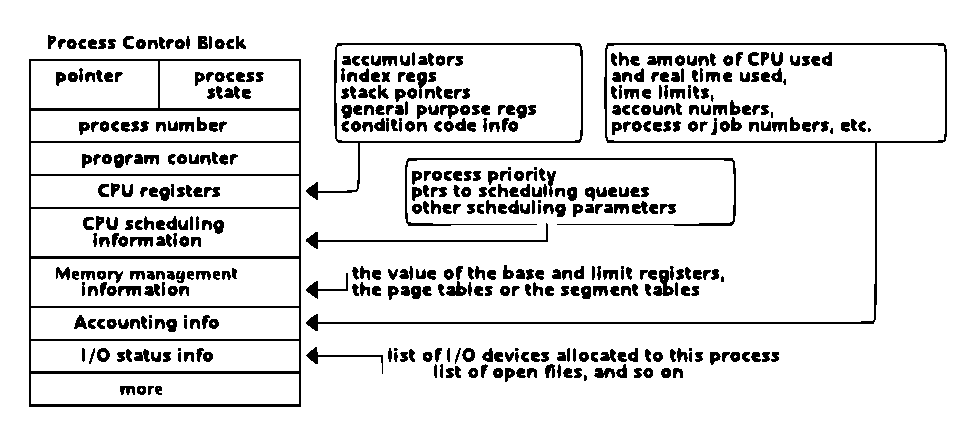
\includegraphics[width=\textwidth]{pcbpdf2}
% 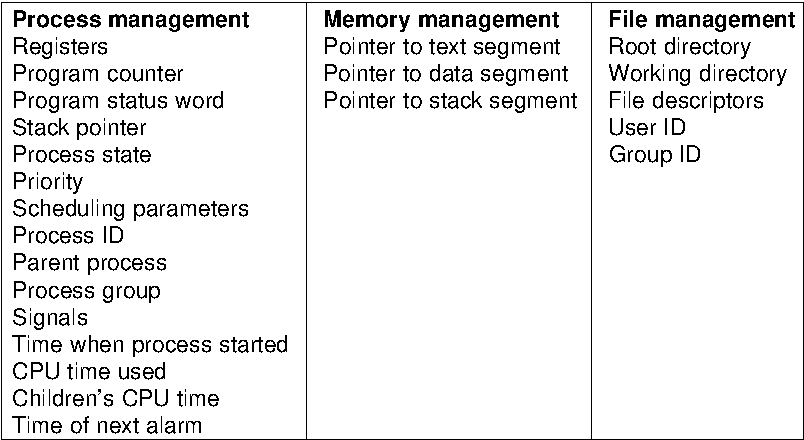
\includegraphics[width=\textwidth]{mos-figs-2-4}

\begin{frame}{Process Control Block (PCB)}
  \begin{minipage}{.7\textwidth}
    \begin{block}{Implementation}
        A process is \alert{the collection of data structures} that fully describes how far
        the execution of the program has progressed.
        \begin{itemize}
        \item Each process is represented by a \alert{PCB}
        \item \texttt{task\_struct} in 
        \end{itemize}
      \end{block}
    \end{minipage}\quad
    \begin{minipage}{.2\textwidth}
      \begin{tblr}{colspec={c},vlines,hlines}
        process state\\
        PID\\
        program counter\\
        registers\\
        memory limits\\
        list of open files\\
        \ldots
      \end{tblr}
    \end{minipage}
\end{frame}

To manage processes, the kernel must have a clear picture of what each process is
doing. It must know, for instance, the process's priority, whether it is running on a CPU
or blocked on an event, what address space has been assigned to it, which files it is
allowed to address, and so on. This is the role of the process descriptor a
\texttt{task\_struct} type structure whose fields contain all the information related to a
single process. As the repository of so much information, the process descriptor is rather
complex. In addition to a large number of fields containing process attributes, the
process descriptor contains several pointers to other data structures that, in turn,
contain pointers to other structures\citetitle[Sec.~3.2, \emph{Process
  Descriptor}]{bovet2005understanding}.

\subsection{Process Creation}
\label{sec:process-creation}

\begin{frame}{Process Creation}
  \begin{center}
    \mode<beamer>{ 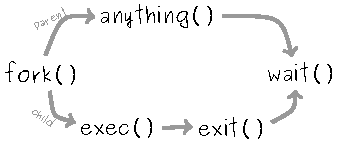
\includegraphics[width=\textwidth]{process-creation} }%
    \mode<article>{ 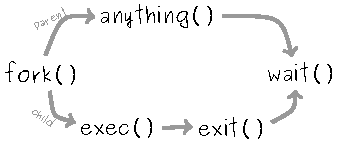
\includegraphics[width=.5\textwidth]{process-creation} }
  \end{center}
  \begin{itemize}
  \item When a process is created, it is almost identical to its parent
    \begin{itemize}
    \item It receives a (logical) copy of the parent's address space, and
    \item executes the same code as the parent
    \end{itemize}
  \item The parent and child have separate copies of the data (stack and heap)
  \end{itemize}
\end{frame}


When a process is created, it is almost identical to its parent. It receives a (logical)
copy of the parent's address space and executes the same code as the parent, beginning at
the next instruction following the process creation system call. Although the parent and
child may share the pages containing the program code (text), they have separate copies of
the data (stack and heap), so that changes by the child to a memory location are invisible
to the parent (and vice versa)\citetitle[Sec.~3.1, \emph{Processes, Lightweight Processes, and
  Threads}]{bovet2005understanding}.

While earlier Unix kernels employed this simple model, modern Unix systems do not. They
support \emph{multi-threaded applications} user programs having many relatively
independent execution flows sharing a large portion of the application data structures. In
such systems, a process is composed of several \emph{user threads} (or simply
\emph{threads}), each of which represents an execution flow of the process. Nowadays, most
multi-threaded applications are written using standard sets of library functions called
\emph{pthread (POSIX thread) libraries}.

Traditional Unix systems treat all processes in the same way: resources owned by the
parent process are duplicated in the child process. This approach makes process creation
very slow and inefficient, because it requires copying the entire address space of the
parent process. The child process rarely needs to read or modify all the resources
inherited from the parent; in many cases, it issues an immediate \texttt{execve()} and
wipes out the address space that was so carefully copied\citetitle[Sec.~3.4, \emph{Creating
  Processes}]{bovet2005understanding}.

Modern Unix kernels solve this problem by introducing three different mechanisms:
\begin{itemize}
\item Copy On Write
\item Lightweight processes
\item The \texttt{vfork()} system call
\end{itemize}


\begin{frame}{Forking in C}
  \begin{center}
    \mode<beamer>{ 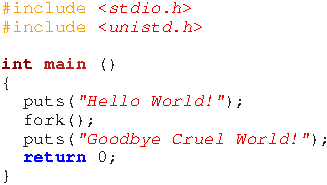
\includegraphics[width=.7\textwidth]{fork-c} }%
    \mode<article>{ \cfile{../src/proc/fork.c} }
  \end{center}
  \begin{itemize}
  \item[\$] \texttt{man fork}
  \end{itemize}
\end{frame}

\begin{frame}{\texttt{exec()}}
  \begin{center}
    \mode<beamer>{ 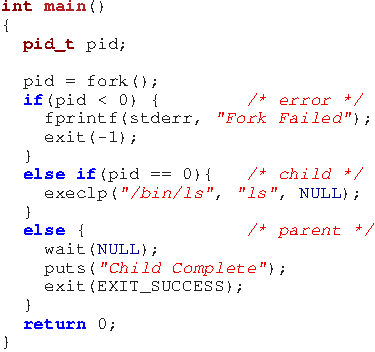
\includegraphics[width=.6\textwidth]{fork-exec-osc-c}}%
    \mode<article>{ \cfile{../src/proc/fork-exec-osc.c}}
  \end{center}
  \begin{itemize}
  \item[\$] \cmd{man 3 exec}
  \end{itemize}
\end{frame}

\subsection{Process State}

\begin{frame}{Process State Transition}
  \begin{center}
    \mode<beamer>{ 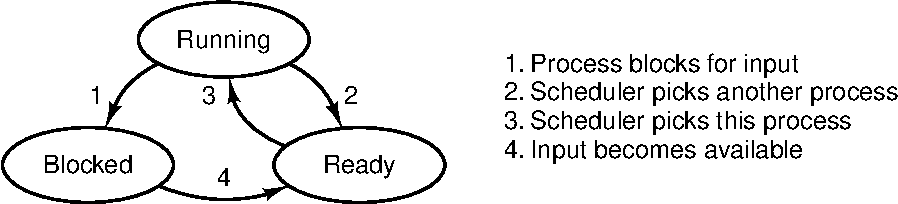
\includegraphics[width=\textwidth]{mos-figs-2-2} }%
    \mode<article>{ 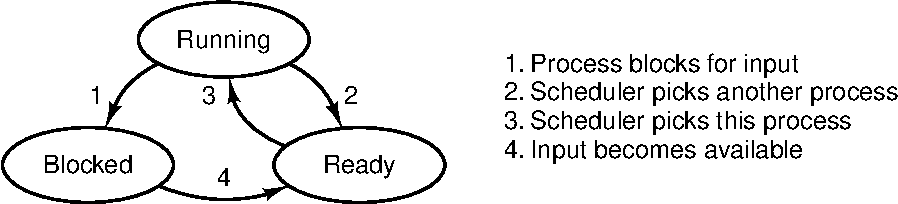
\includegraphics[width=.7\textwidth]{mos-figs-2-2} }
  \end{center}
\end{frame}

See also: \citetitle[Sec.~3.2.1, \emph{Process State}]{bovet2005understanding}.

\subsection{CPU Switch From Process To Process}
\label{sec:cpu-switch-from}

\begin{frame}{CPU Switch From Process To Process}
  \mode<beamer>{\centering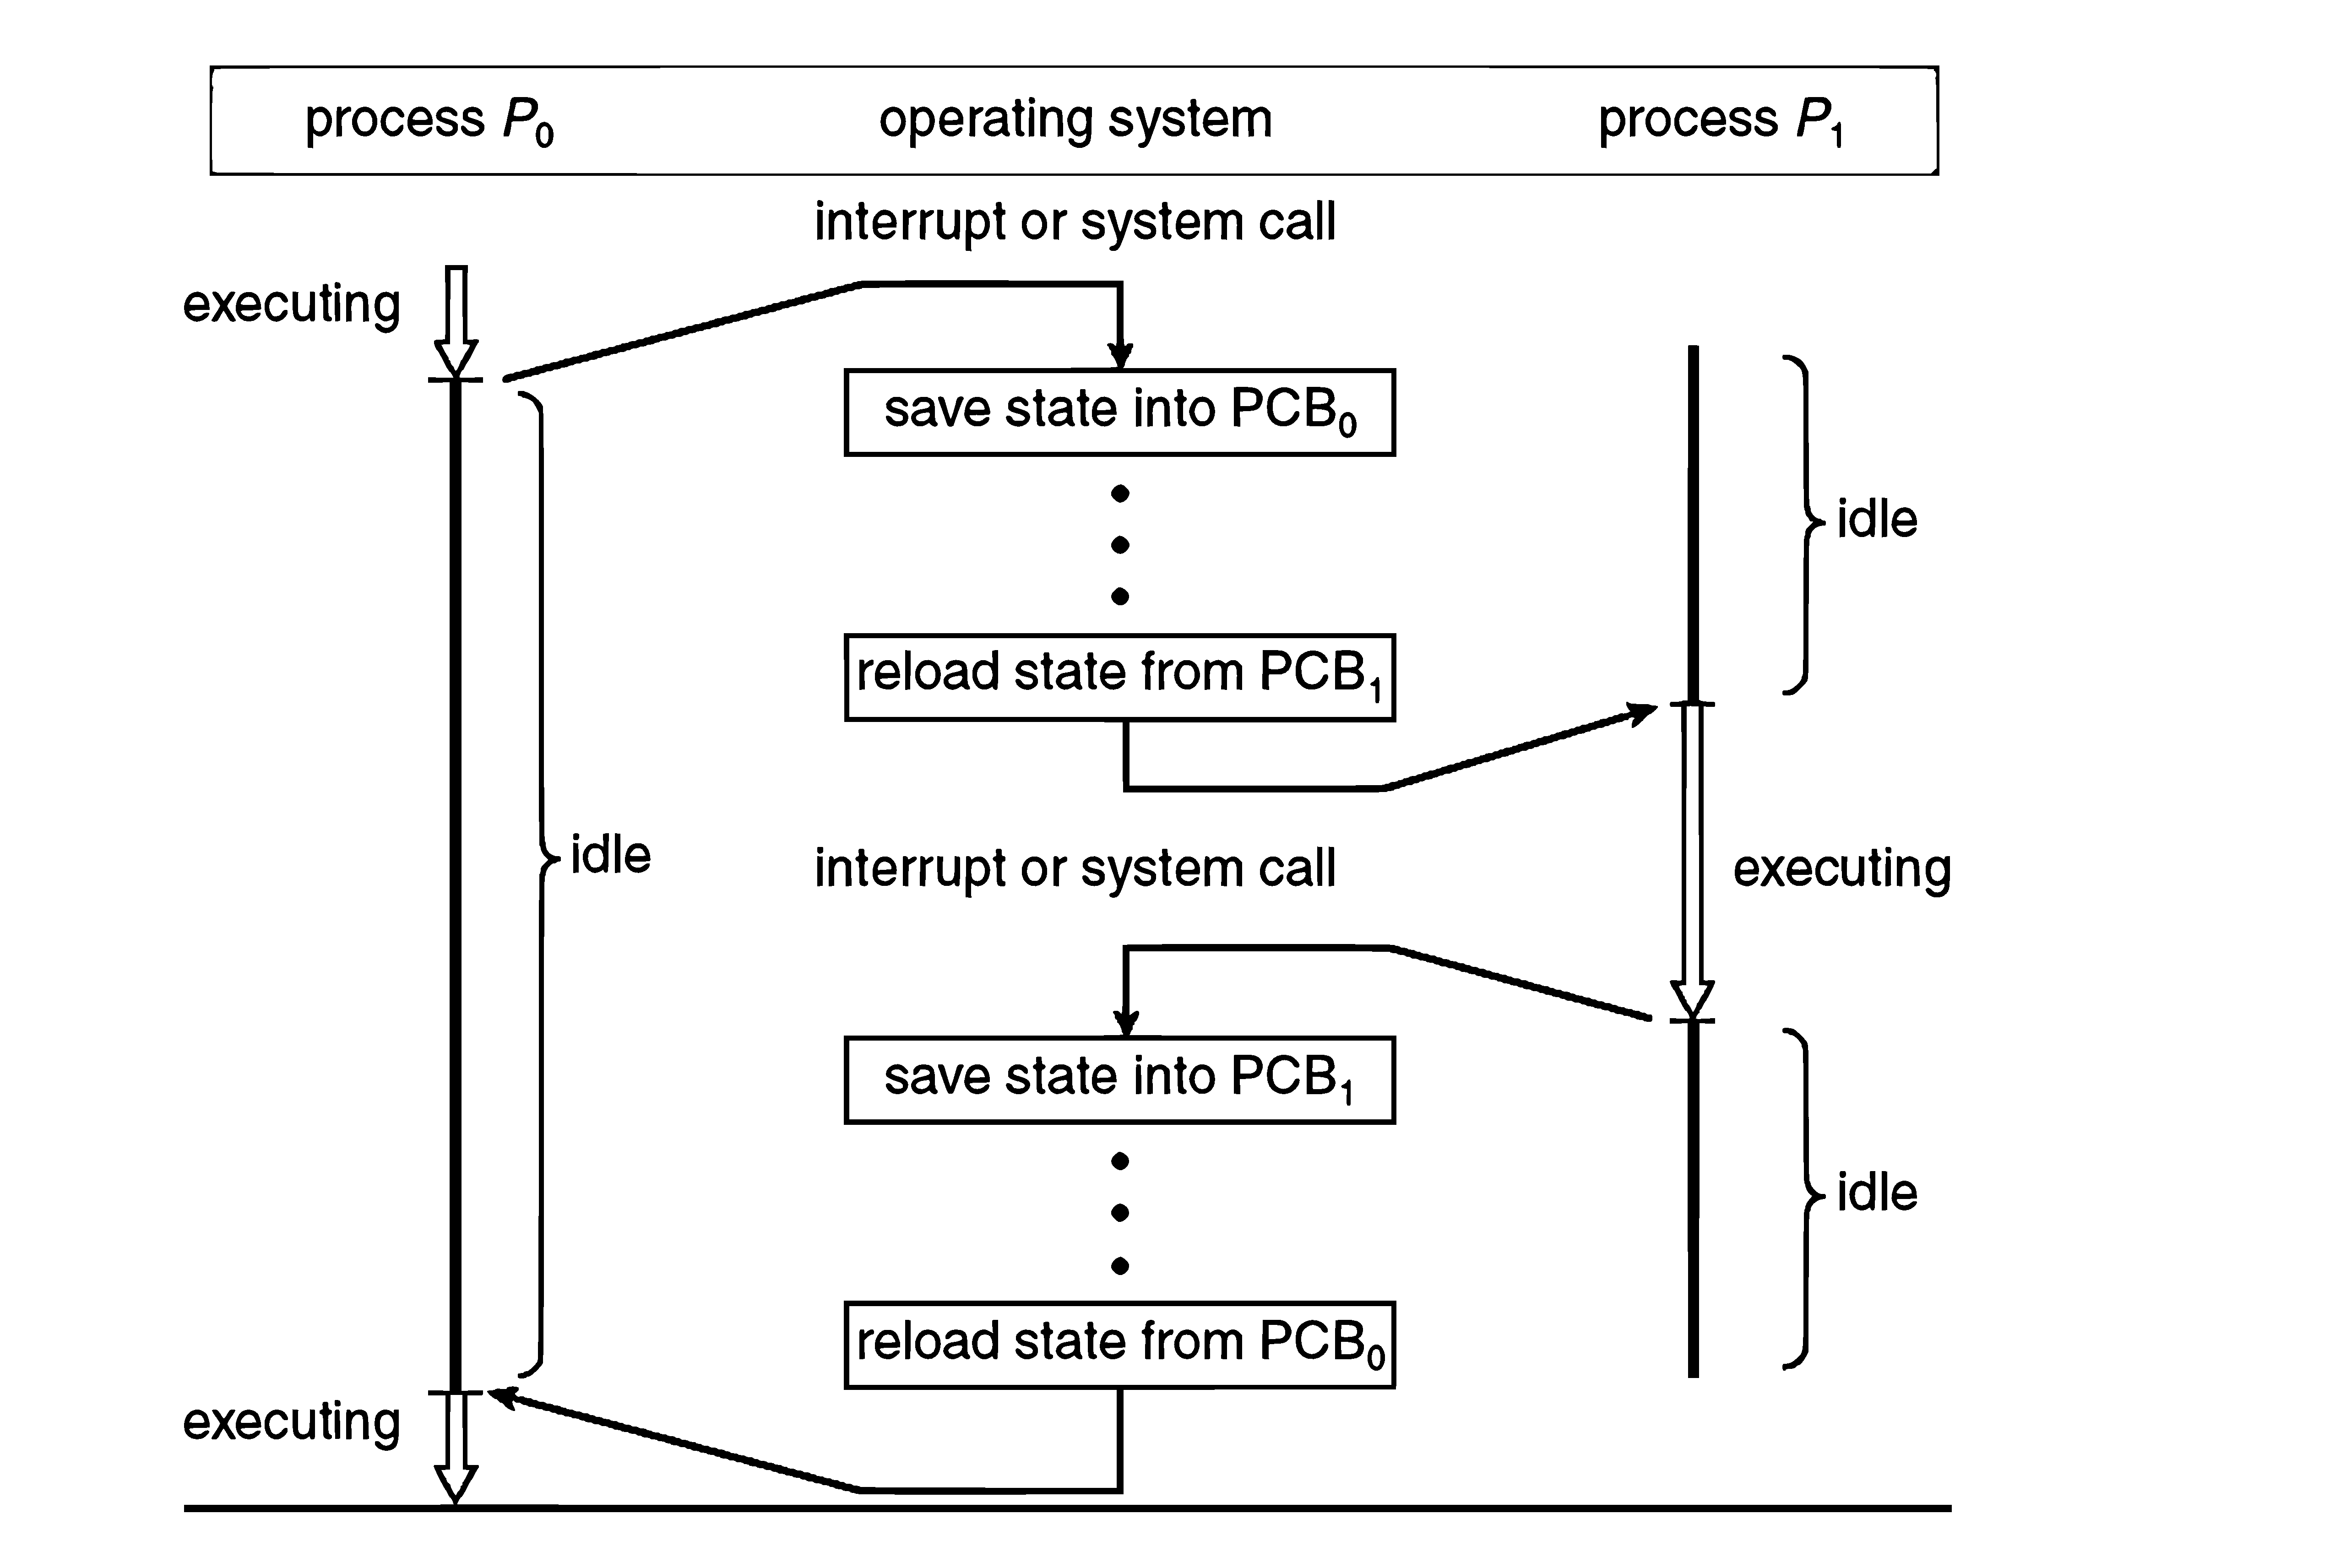
\includegraphics[height=.9\textheight]{cpu-switch} }%
  \mode<article>{\centering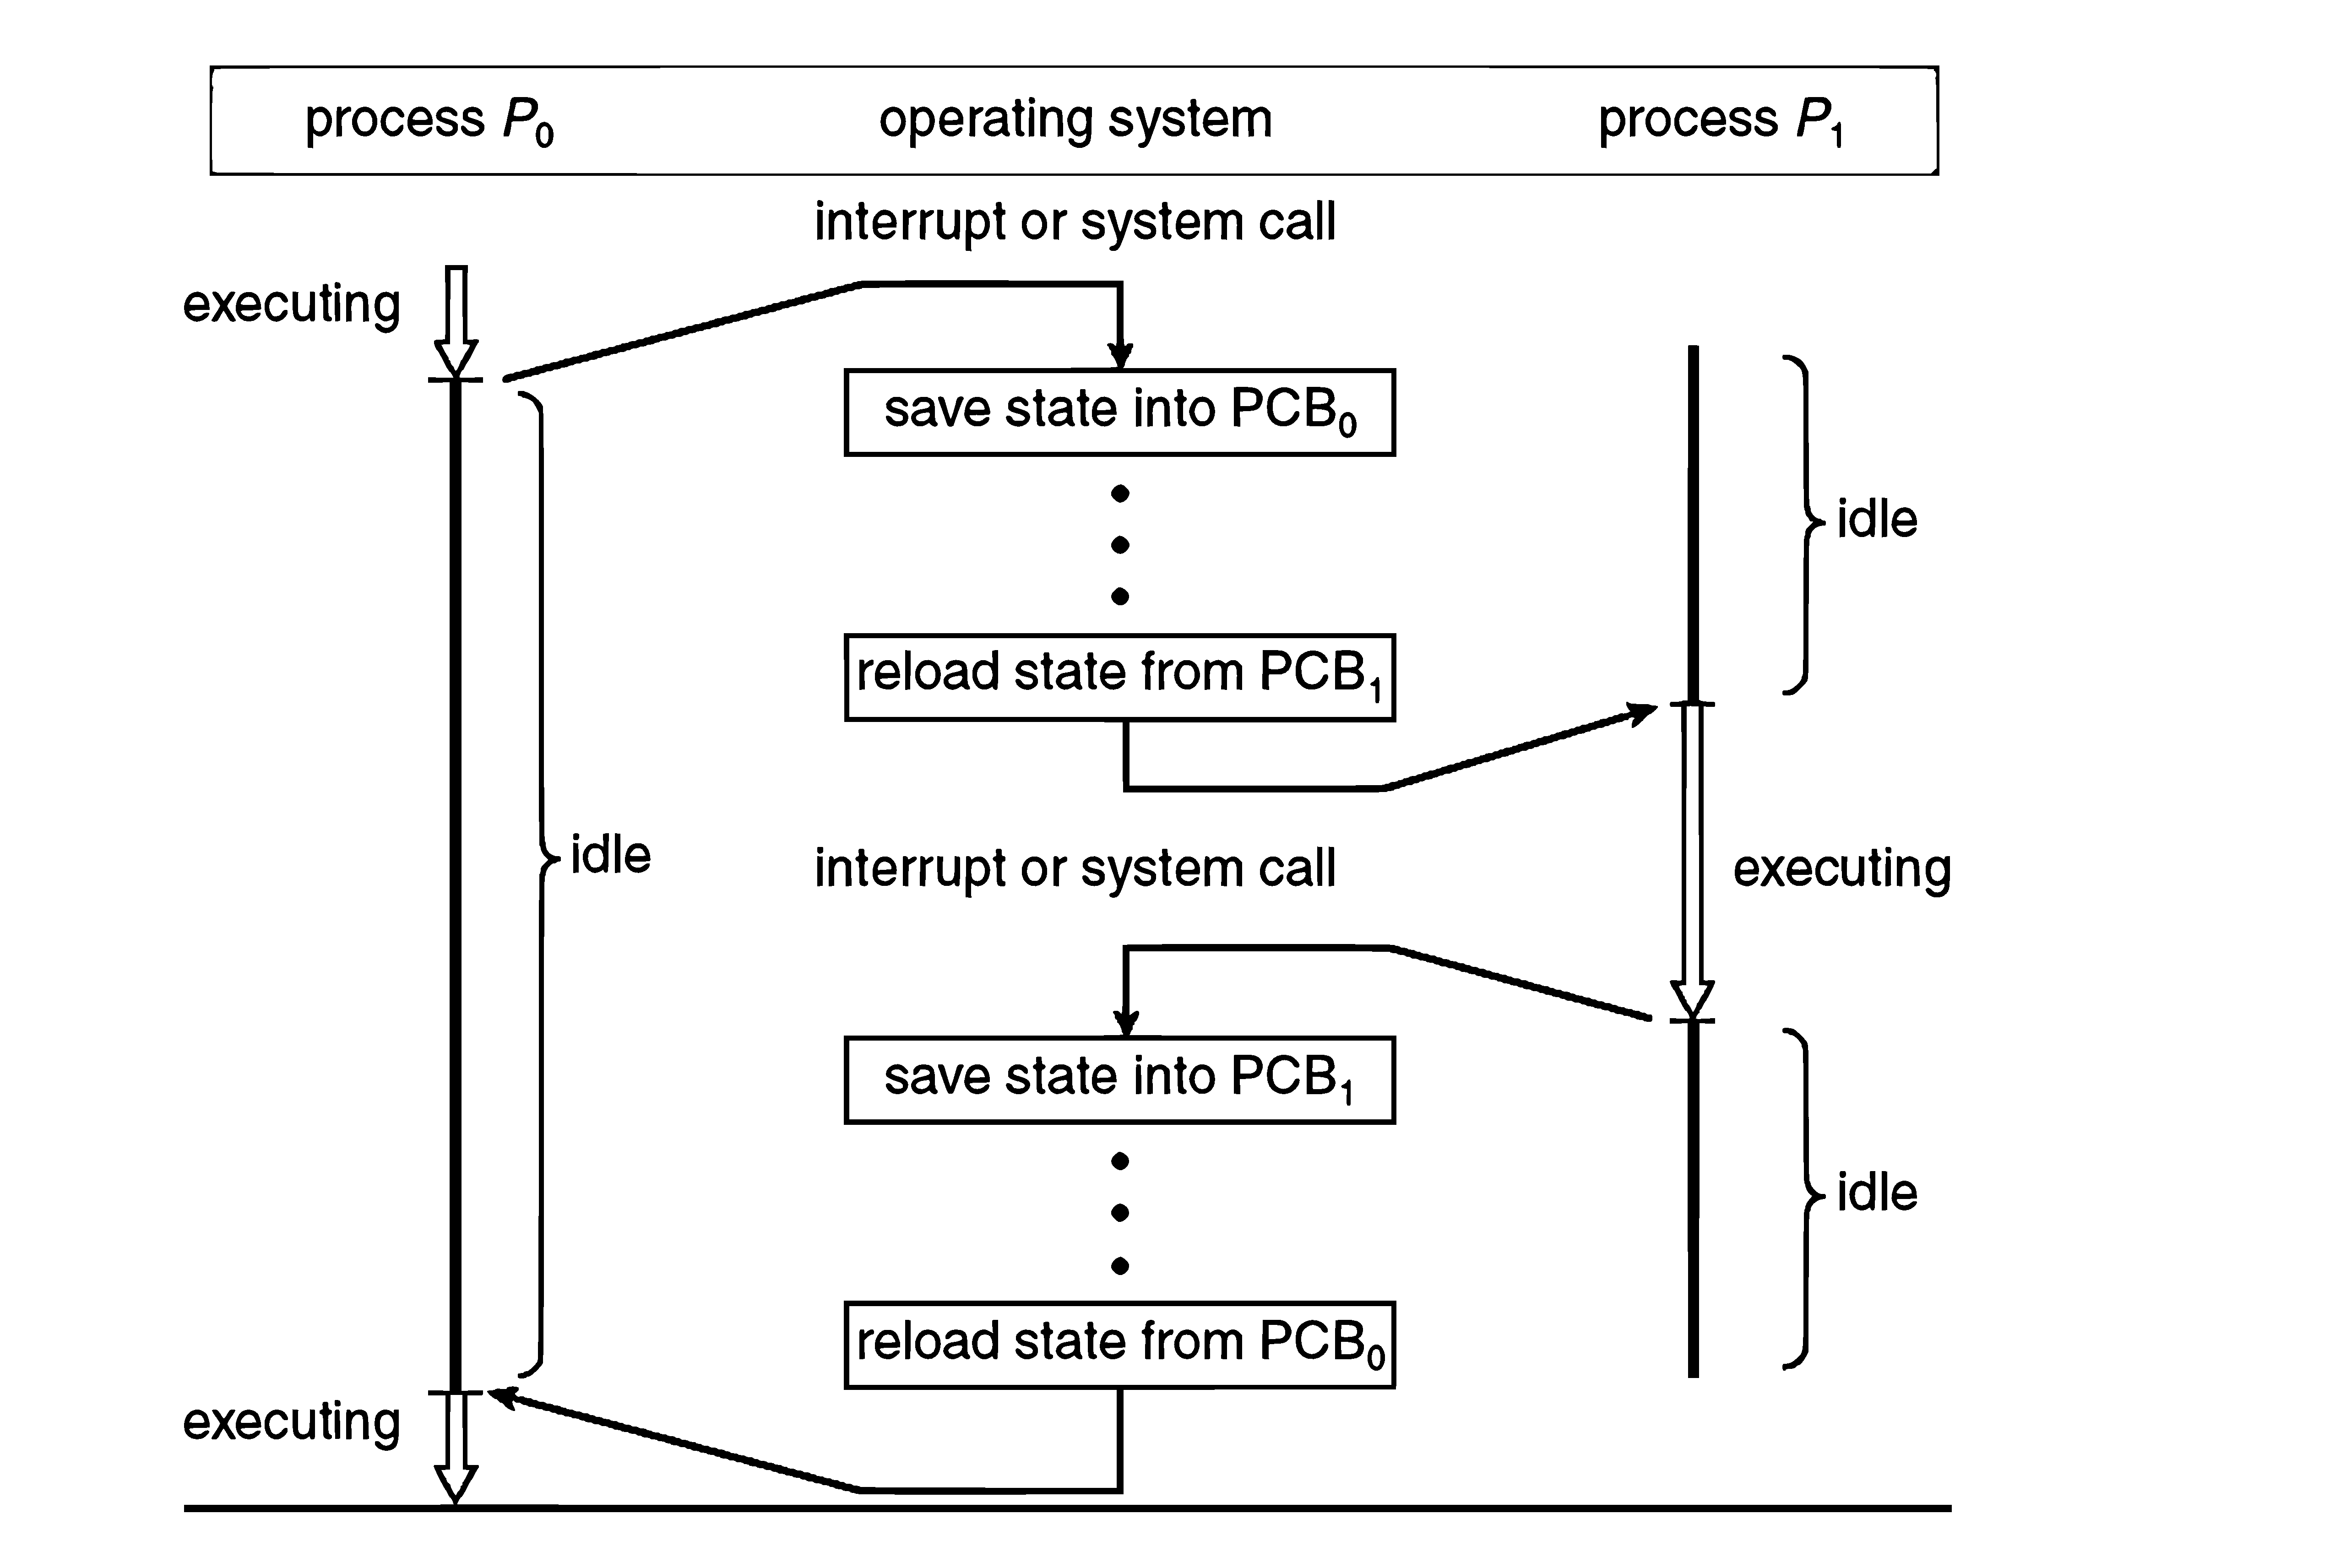
\includegraphics[width=.7\textwidth]{cpu-switch} }
\end{frame}

See also: \citetitle[Sec.~3.3, \emph{Process Switch}]{bovet2005understanding}.


\section{Threads}
\label{sec:threads}

\subsection{Processes vs. Threads}
\label{sec:proc-vs.-thre}

\begin{frame}{Process vs. Thread}
    \begin{tblr}{rcl}
      a single-threaded process&=&resource + execution\\
      a  multi-threaded process&=&resource + executions\\
    \end{tblr}
    \begin{center}
      \mode<beamer>{ 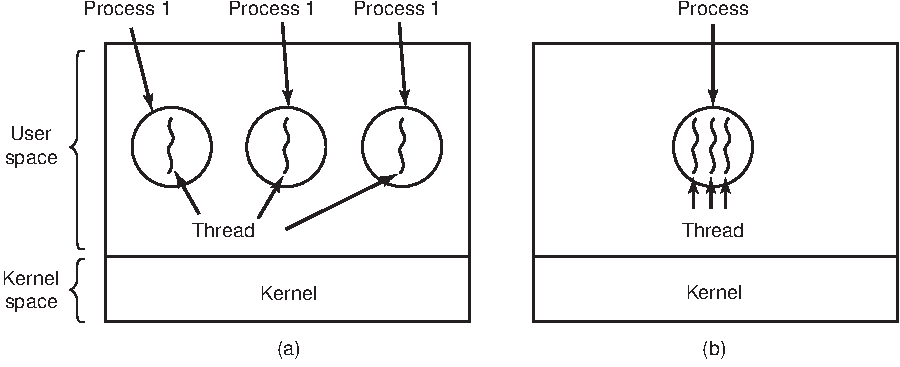
\includegraphics[width=.7\textwidth]{mos-figs-2-6} }%
      \mode<article>{ 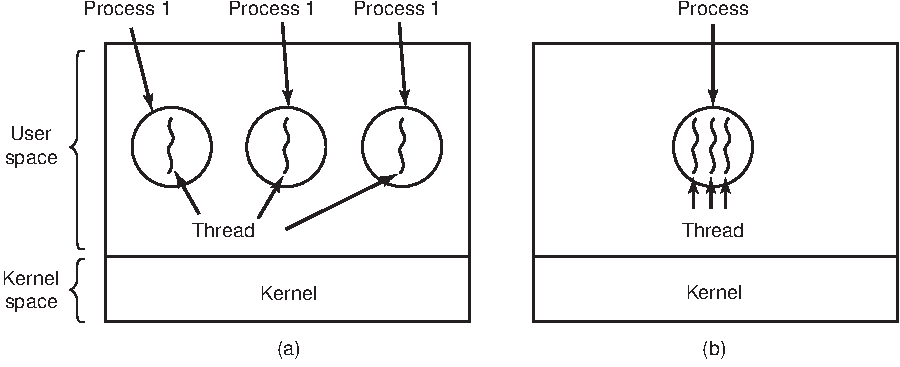
\includegraphics[width=.6\textwidth]{mos-figs-2-6} }
    \end{center}
  \begin{description}
  \item[A process] = a unit of resource ownership, used to group resources together
  \item[A thread] = a unit of scheduling, scheduled for execution on the CPU
  \end{description}  
\end{frame}

\begin{frame}{Process vs. Thread}
  \begin{center}
    \begin{tblr}{width=.9\textwidth,colspec={X|X},row{1}={font=\bfseries}}
      {multiple threads running in one process:}&
      {multiple processes running in one computer:}\\
      share an address space and other resources&
      share physical memory, disk, printers \ldots\\
    \end{tblr}
  \end{center}
  \begin{block}{No protection between threads}
    \begin{description}
    \item[impossible] --- because process is the minimum unit of resource management
    \item[unnecessary] --- a process is owned by a single user
    \end{description}    
  \end{block}
\end{frame}

\begin{frame}{Threads}
  \begin{center}
    \begin{tblr}{colspec={ccc},vlines,hlines,cell{1}{1}={c=3}{c}}
      code, data, open files, signals\ldots&&\\
      thread ID&thread ID&thread ID\\
      {program\\counter}&{program\\counter}&{program\\counter}\\
      {register\\set}&{register\\set}&{register\\set}\\
      stack&stack&stack\\
    \end{tblr}
    % \mode<beamer>{ 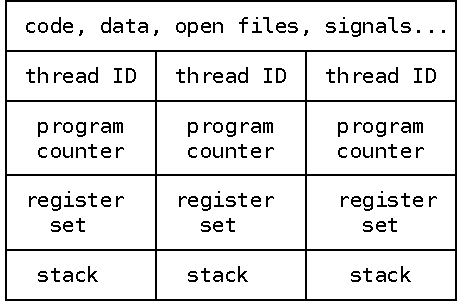
\includegraphics[width=.8\textwidth]{thread-components} }%
    % \mode<article>{ 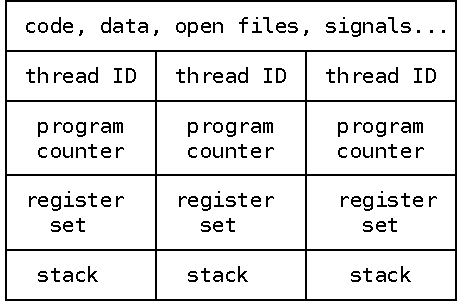
\includegraphics[width=.4\textwidth]{thread-components} }
  \end{center}
\end{frame}

\subsection{Why Thread?}
\label{sec:why-thread}

\begin{frame}{A Multi-threaded Web Server}\label{webserver}
  \begin{center}
    \mode<beamer>{ 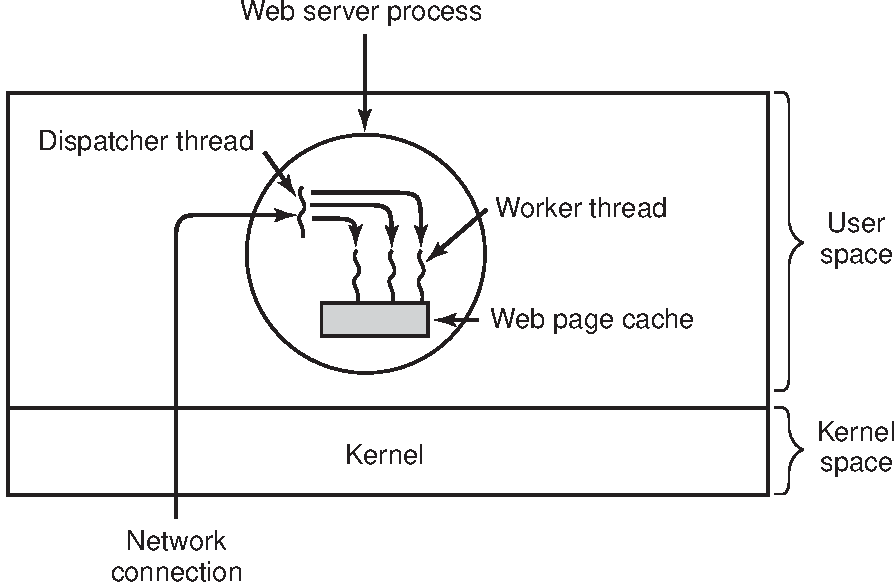
\includegraphics[width=.6\textwidth]{mos-figs-2-10} }%
    \mode<article>{ 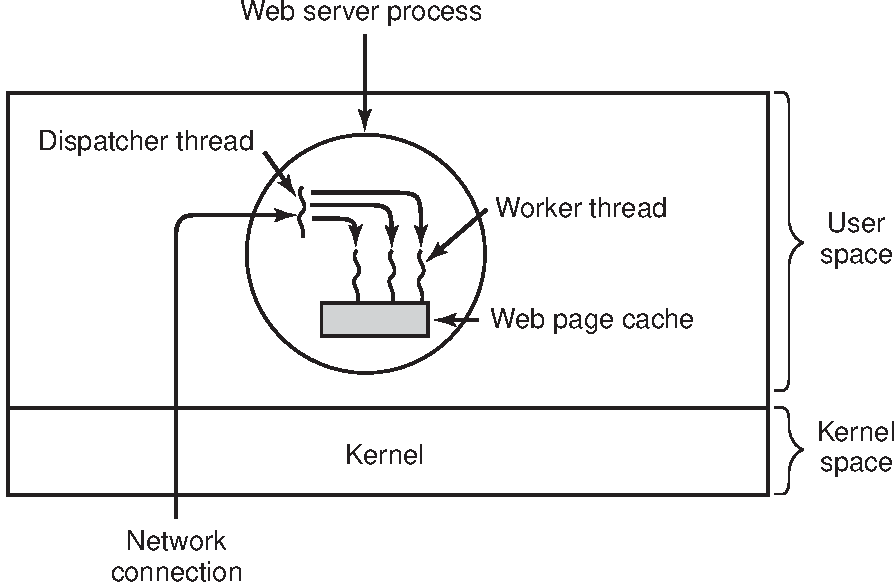
\includegraphics[width=.5\textwidth]{mos-figs-2-10} }
  \end{center}
  \begin{center}
    \mode<beamer>{ 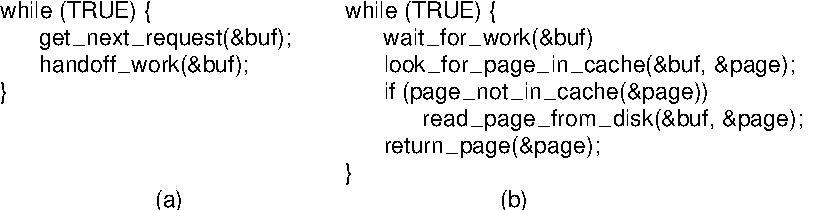
\includegraphics[width=.75\textwidth]{mos-figs-2-11} }%
    \mode<article>{ 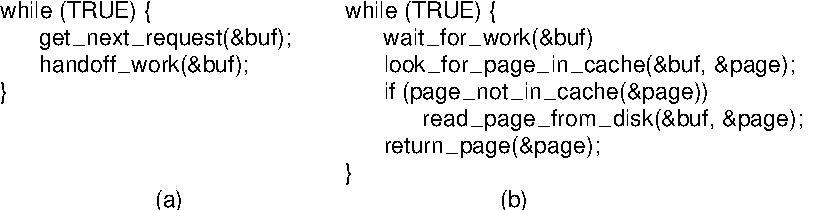
\includegraphics[width=.6\textwidth]{mos-figs-2-11} }
  \end{center}
\end{frame}

\begin{frame}{A Word Processor With 3 Threads}
  \begin{center}
    \mode<beamer>{ 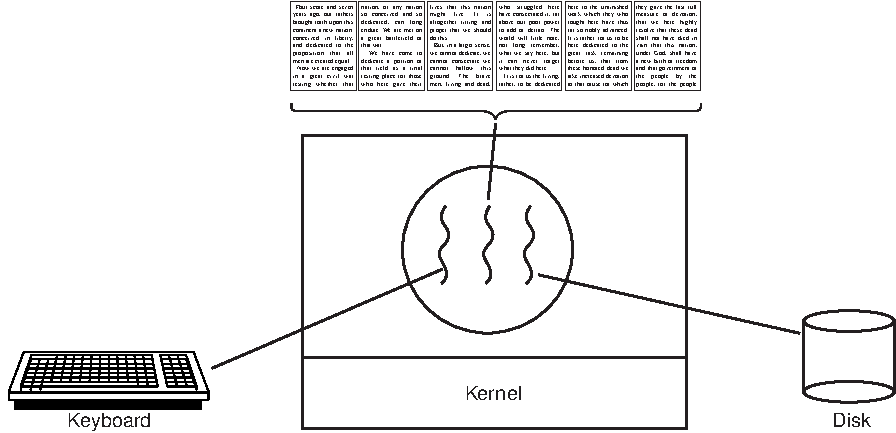
\includegraphics[width=\textwidth]{mos-figs-2-9} }%
    \mode<article>{ 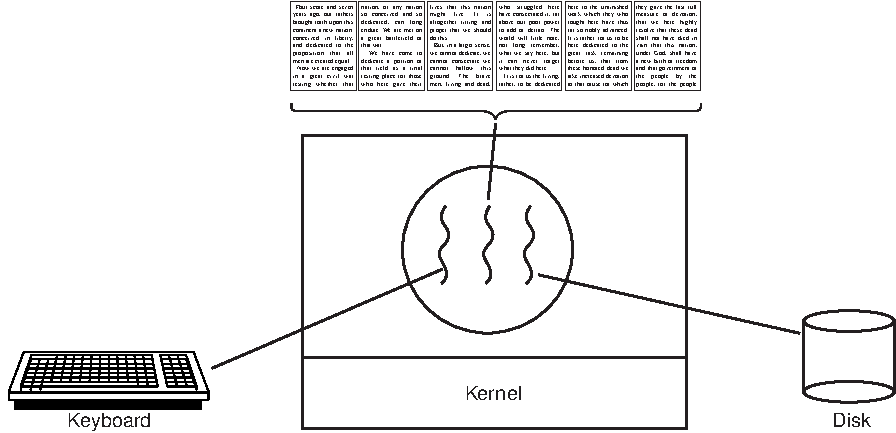
\includegraphics[width=.6\textwidth]{mos-figs-2-9} }
  \end{center}
\end{frame}

\begin{frame}{Why Having a Kind of Process Within a Process?}{}
  \begin{itemize}
  \item Responsiveness
    \begin{itemize}
    \item Good for interactive applications.
    \item A process with multiple threads makes a great server (e.g. a web server):
      \begin{itemize}
      \item[] Have one server process, many "worker" threads -- if one thread blocks (e.g. on a
        read), others can still continue executing
      \end{itemize}
    \end{itemize}
  \item Economy -- Threads are cheap!
    \begin{itemize}
    \item Cheap to create -- only need a stack and storage for registers
    \item Use very little resources -- don't need new address space, global data, program code, or
      OS resources
    \item switches are fast -- only have to save/restore PC, SP, and registers
    \end{itemize}
  \item Resource sharing -- Threads can pass data via shared memory; no need for IPC
    \item Can take advantage of multiprocessors
  \end{itemize}
\end{frame}

\subsection{Thread Characteristics}
\label{sec:thread-char}

\begin{frame}{Thread States Transition}{Same as process states transition}
  \begin{center}
    \mode<beamer>{ 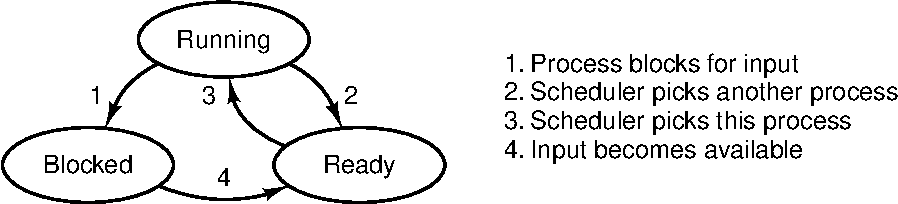
\includegraphics[width=\textwidth]{mos-figs-2-2} }%
    \mode<article>{ 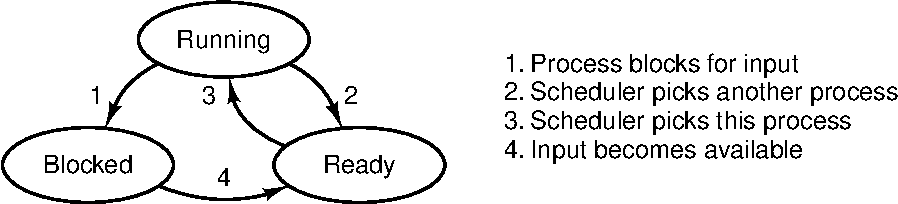
\includegraphics[width=.6\textwidth]{mos-figs-2-2} }
  \end{center}
\end{frame}

\begin{frame}{Each Thread Has Its Own Stack}
  \begin{itemize}
  \item A typical stack stores local data and call information for (usually nested) procedure
    calls. 
  \item Each thread generally has a different execution history.
  \end{itemize}
  \begin{center}
    \mode<beamer>{ 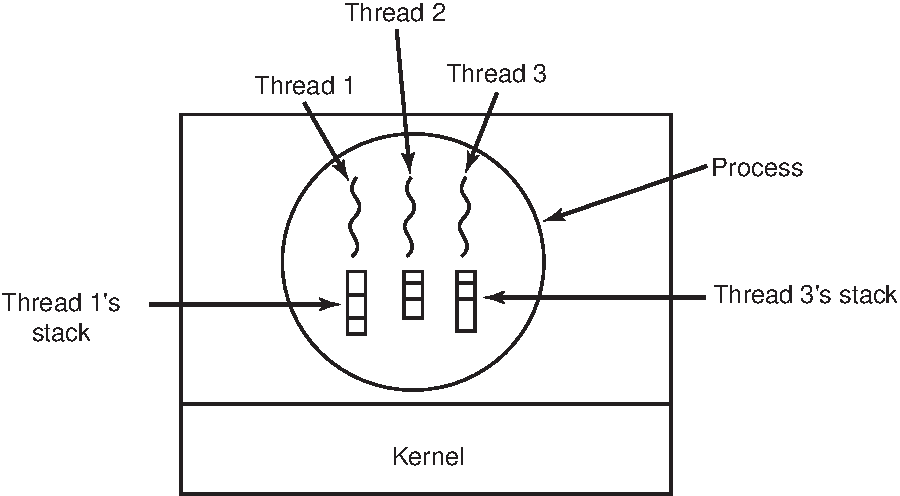
\includegraphics[width=.8\textwidth]{mos-figs-2-8} }%
    \mode<article>{ 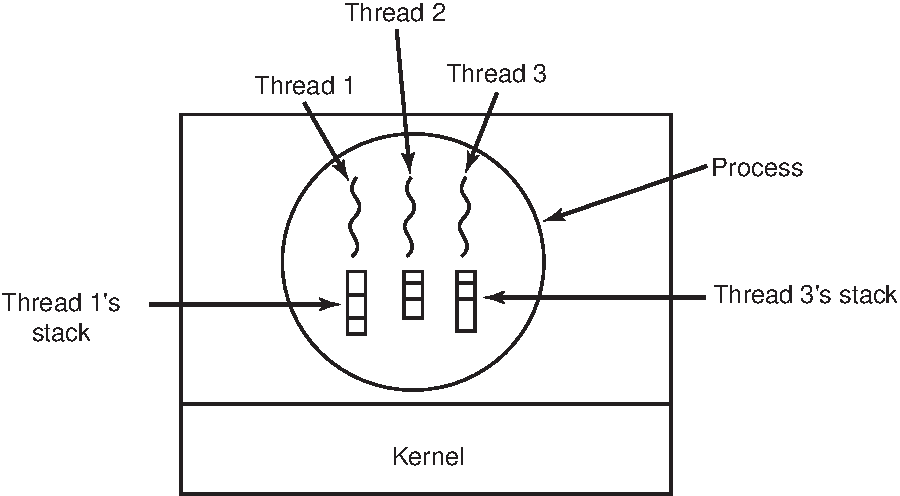
\includegraphics[width=.6\textwidth]{mos-figs-2-8} }
  \end{center}
\end{frame}

\begin{frame}{Thread Operations}
  \begin{center}
    \mode<beamer>{ 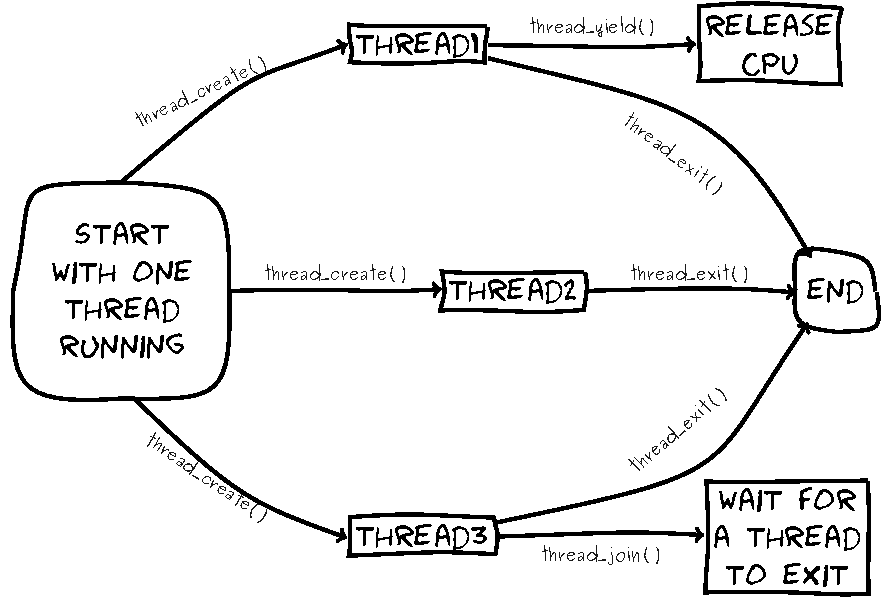
\includegraphics[width=.8\textwidth]{thread-operations} }%
    \mode<article>{ 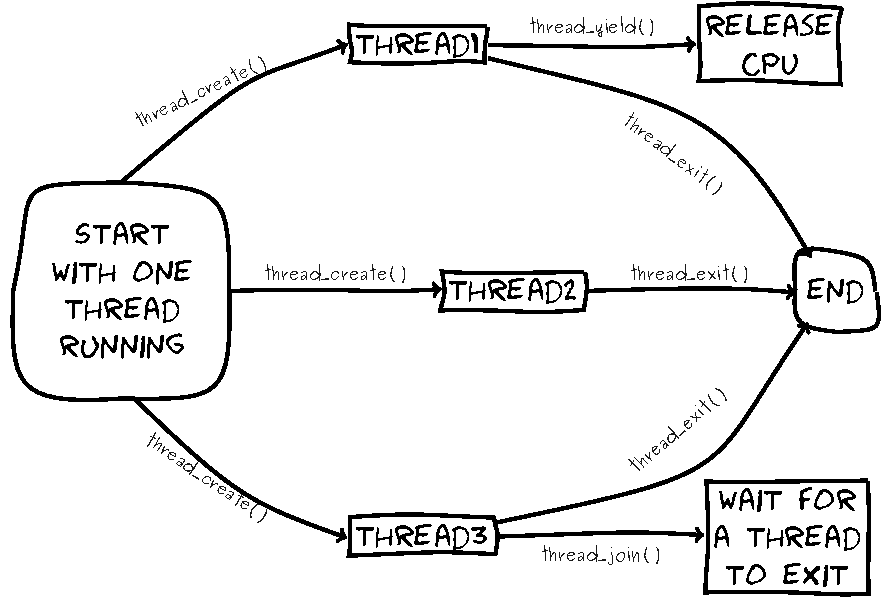
\includegraphics[width=.6\textwidth]{thread-operations} }
  \end{center}
\end{frame}

\subsection{POSIX Threads}
\label{sec:posix-threads}

\begin{frame}{POSIX Threads}
  \begin{description}
  \item[IEEE 1003.1c] The standard for writing portable threaded programs. The threads package it
    defines is called \alert{Pthreads}, including over 60 function calls, supported by most UNIX
    systems.
  \end{description}
  \begin{block}{Some of the Pthreads function calls}
    \begin{center}{\small
        \begin{tblr}{colspec={ll},hline{1,2,Z},%
            row{1}={c,font=\bfseries},%
          cell{2-Z}{1}={font=\ttfamily}}
        Thread call&Description\\
        pthread\_create()&Create a new thread\\
        pthread\_exit()&Terminate the calling thread\\
        pthread\_join()&Wait for a specific thread to exit\\
        pthread\_yield()&Release the CPU to let another thread run\\
        pthread\_attr\_init()&Create and initialize a thread's attribute structure\\
        pthread\_attr\_destroy()&Remove a thread's attribute structure\\
      \end{tblr}}
    \end{center}
  \end{block}
\end{frame}

\begin{frame}{Pthreads}{Example 1}
  \mode<beamer>{ \centering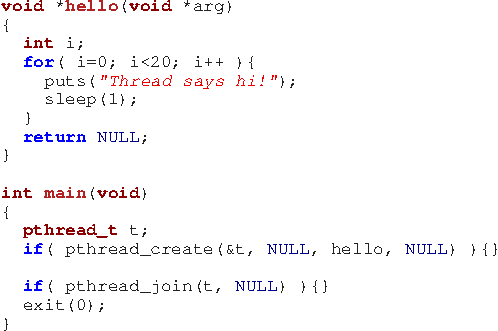
\includegraphics[width=.8\textwidth]{thread1-c} }%
  \mode<article>{\cfile{../src/proc/thread1.c}}
\end{frame}

See also:
\begin{itemize}
\item IBM Developworks: POSIX threads
  explained\footnote{\url{http://www.ibm.com/developerworks/linux/library/l-posix1/index.html}}.
\item stackoverflow.com: What is the difference between \texttt{exit()} and
  \texttt{abort()}?\footnote{\url{http://stackoverflow.com/questions/397075/what-is-the-difference-between-exit-and-abort}}.
\end{itemize}

\begin{frame}{Pthreads}
  \begin{description}
  \item[\texttt{pthread\_t}] defined in \texttt{pthread.h}, is often called a ``thread id''
    (\texttt{tid});
  \item[\texttt{pthread\_create()}] returns zero on success and a non-zero value on failure;
  \item[\texttt{pthread\_join()}] returns zero on success and a non-zero value on failure;
  \end{description}
  \begin{block}{How to use pthread?}
    \begin{itemize}
    \item[] \texttt{\#include<pthread.h>}
    \item[\$] \texttt{gcc thread1.c -o thread1 -pthread}
    \item[\$] \texttt{./thread1}
    \end{itemize}
  \end{block}
\end{frame}

\begin{frame}{Pthreads}{Example 2}
  \begin{center}
    \mode<beamer>{ 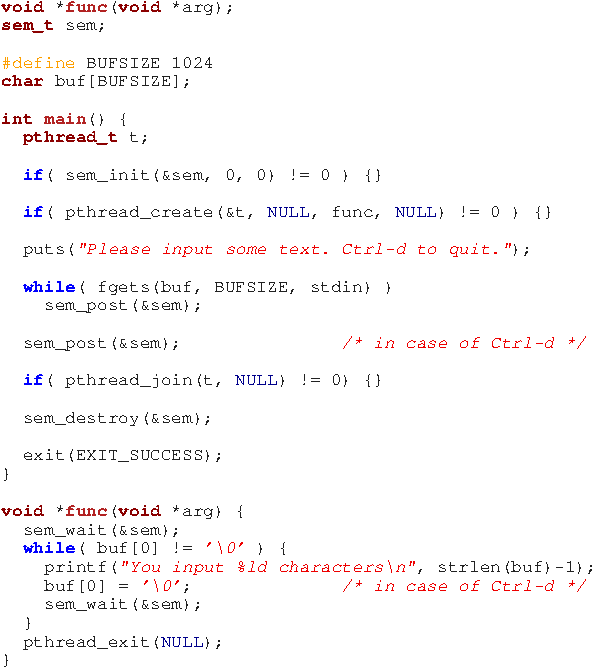
\includegraphics[height=.88\textheight]{thread3} }%
    \mode<article>{\cfile{../src/proc/thread3.c}}
  \end{center}
\end{frame}

% \begin{frame}{Pthreads}
%   With or without \texttt{pthread\_join()}? Check it by yourself.
% \end{frame}

\subsection{User-Level Threads vs. Kernel-level Threads}
\label{sec:user-threads-vs}

\begin{frame}{User-Level Threads vs. Kernel-Level Threads}
  \begin{center}
    \mode<beamer>{ 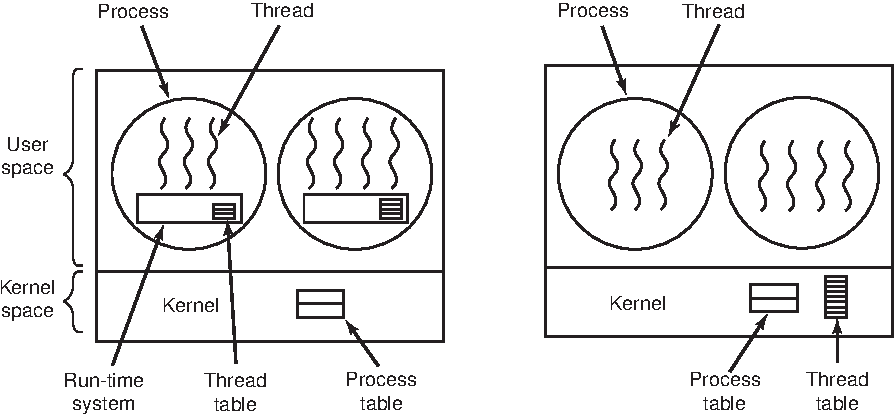
\includegraphics[width=\textwidth]{mos-figs-2-13} }%
    \mode<article>{ 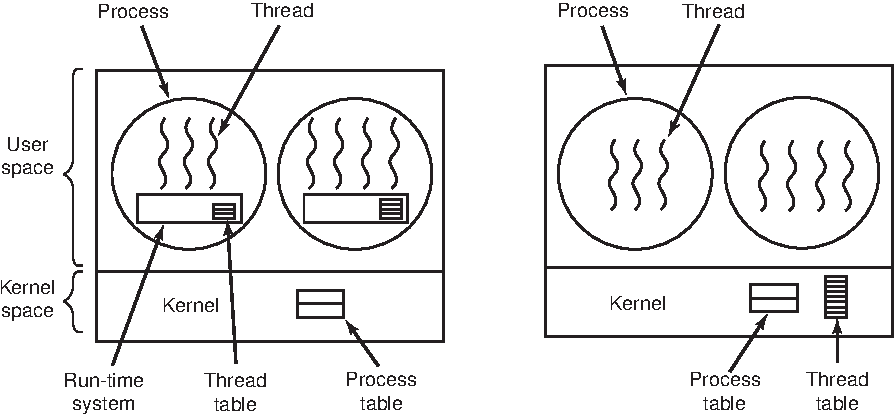
\includegraphics[width=.6\textwidth]{mos-figs-2-13} }
  \end{center}
\end{frame}

\begin{frame}{User-Level Threads}
  \begin{description}
  \item[User-level threads] provide a library of functions to allow user processes to create and
    manage their own threads.
  \end{description}
  \begin{itemize}
  \item[☺] No need to modify the OS\\[-.5ex]
  \item[☺] Simple representation\\[-.5ex]
    \begin{itemize}
    \item each thread is represented simply by a PC, regs, stack, and a small TCB, all
        stored in the user process' address space
    \end{itemize}
  \item[☺] Simple Management\\[-.5ex]
    \begin{itemize}
    \item creating a new thread, switching between threads, and synchronization between threads can
      all be done without intervention of the kernel
    \end{itemize}
  \item[☺] Fast\\[-.5ex]
    \begin{itemize}
    \item thread switching is not much more expensive than a procedure call
    \end{itemize}
  \item[☺] Flexible\\[-.5ex]
    \begin{itemize}
    \item CPU scheduling (among threads) can be customized to suit the needs of the algorithm --
      each process can use a different thread scheduling algorithm
    \end{itemize}
  \end{itemize}
\end{frame}

\begin{frame}{User-Level Threads}
  \begin{itemize}
  \item[\alert{☹}]  Lack of coordination between threads and OS kernel
    \begin{itemize}
    \item Process as a whole gets one time slice
    \item Same time slice, whether process has 1 thread or 1000 threads
    \item Also -- up to each thread to relinquish control to other threads in that process
    \end{itemize}
  \item[\alert{☹}] Requires non-blocking system calls (i.e. a multithreaded kernel)
    \begin{itemize}
    \item Otherwise, entire process will blocked in the kernel, even if there are runnable threads
      left in the process
    \item part of motivation for user-level threads was not to have to modify the OS
    \end{itemize}
  \item[\alert{☹}] If one thread causes a page fault (interrupt!), the entire process
    blocks
  \end{itemize}
\end{frame}

See also: \emph{More about blocking and non-blocking calls}\footnote{\url{http://www.daniweb.com/software-development/computer-science/threads/384575/synchronous-vs-asynchronous-blocking-vs-non-blocking}}.

\begin{frame}{Kernel-Level Threads}
  \begin{description}
  \item[Kernel-level threads] kernel provides system calls to create and manage threads
  \end{description}
  \begin{itemize}
  \item[☺] Kernel has full knowledge of all threads
    \begin{itemize}
    \item Scheduler may choose to give a process with 10 threads more time than process with only 1
      thread
    \end{itemize}
  \item[☺] Good for applications that frequently block (e.g. server processes with
    frequent interprocess communication)
  \item[\alert{☹}] Slow -- thread operations are 100s of times slower than for
    user-level threads
  \item[\alert{☹}] Significant overhead and increased kernel complexity --- kernel must
    manage and schedule threads as well as processes
    \begin{itemize}
    \item Requires a full thread control block (TCB) for each thread
    \end{itemize}
  \end{itemize}
\end{frame}

\begin{frame}<beamer>{Hybrid Implementations}{Combine the advantages of two}
  \centering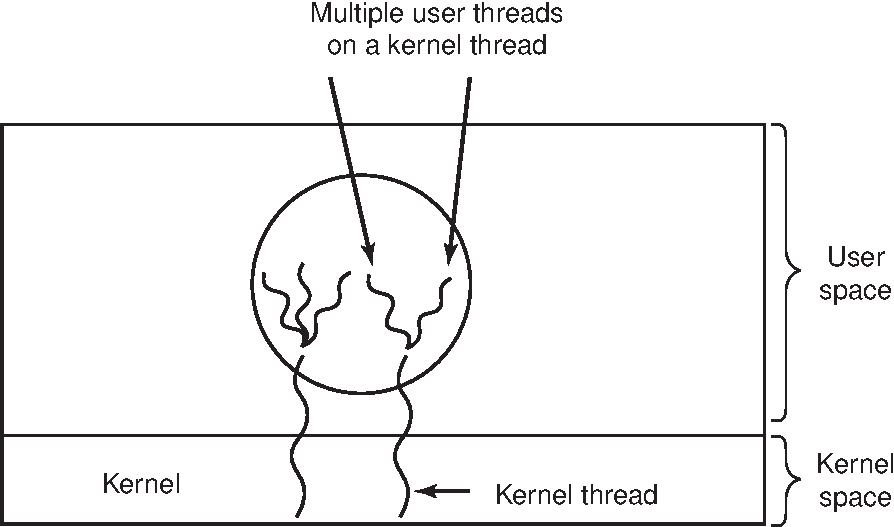
\includegraphics[width=.8\textwidth]{mos-figs-2-14}
\end{frame}

\begin{center}
  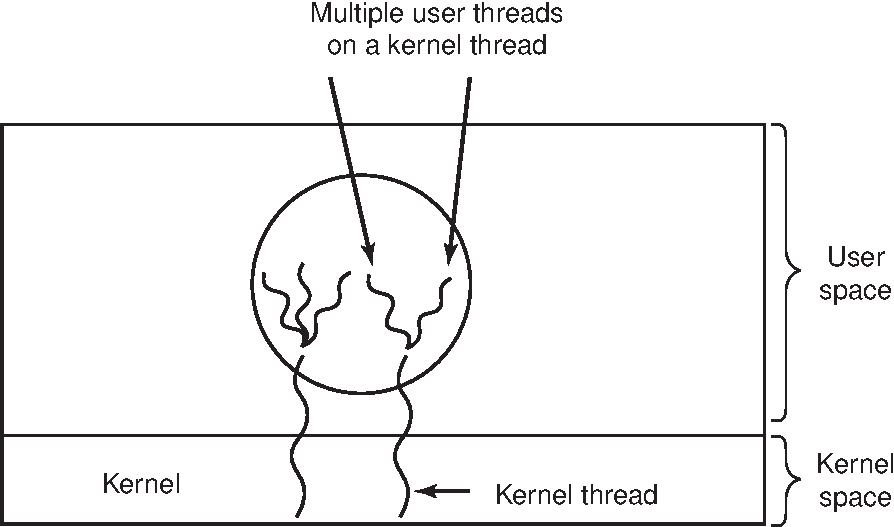
\includegraphics[width=.5\textwidth]{mos-figs-2-14}
\end{center}
% \begin{frame}{Two-Level Thread Model}{Digital UNIX, Solaris, IRIX, HP-UX}
%   \begin{center}
%     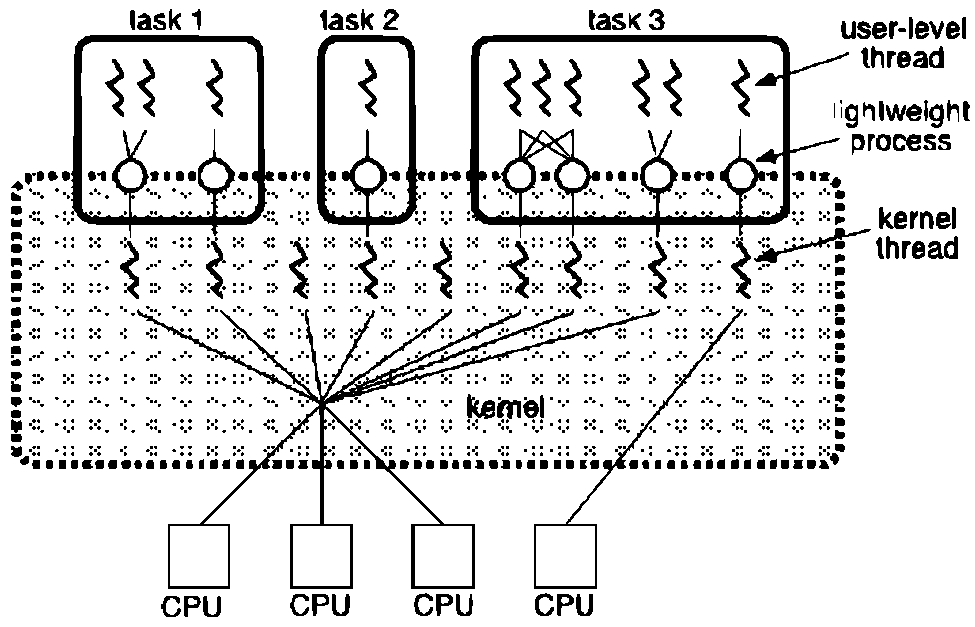
\includegraphics[width=\textwidth]{thread-walker}
%   \end{center}
% \end{frame}

% \begin{frame}{Two-Level Thread Model}{Digital UNIX, Solaris, IRIX, HP-UX}
%   \begin{itemize}
%   \item User-level threads for user processes
%     \begin{itemize}
%     \item Lightweight process (LWP) serves as a "virtual CPU" where user threads can run
%     \end{itemize}
%   \item Kernel-level threads for use by kernel
%     \begin{itemize}
%     \item One for each LWP
%     \item Others perform tasks not related to LWPs
%     \item OS supports multiprocessor systems
%     \end{itemize}
%   \end{itemize}
% \end{frame}

\begin{frame}{Programming Complications}
  \begin{itemize}
  \item \texttt{fork()}: shall the child has the threads that its parent has?
  \item What happens if one thread closes a file while another is still reading from it?
  \item What happens if several threads notice that there is too little memory?
  \end{itemize}
  \alert{And sometimes, threads fix the symptom, but not the problem.}
\end{frame}

\subsection{Linux Threads}
\label{sec:linux-threads}

\begin{frame}{Linux Threads}
  \begin{block}{To the Linux kernel, there is no concept of a thread}
    \begin{itemize}
    \item Linux implements all threads as standard processes
    \item To Linux, a thread is merely a process that shares certain resources with other
      processes
    \item Some OS (MS Windows, Sun Solaris) have cheap threads and expensive processes
    \item Linux processes are already quite lightweight\par
      On a \unit[75]{MHz} Pentium
      \begin{tblr}{r@{\;}l}
        thread:& \unit[1.7]{\mu{}s}\\
        fork:& \unit[1.8]{\mu{}s}
      \end{tblr}
    \end{itemize}
  \end{block}
\end{frame}


\citetitle[Sec.~3.1, \emph{Processes, Lightweight Processes, and
  Threads}]{bovet2005understanding} Older versions of the Linux kernel offered no support
for multithreaded applications. From the kernel point of view, a multithreaded application
was just a normal process. The multiple execution flows of a multithreaded application
were created, handled, and scheduled entirely in User Mode, usually by means of a
POSIX-compliant \emph{pthread} library.

However, such an implementation of multithreaded applications is not very
satisfactory. For instance, suppose a chess program uses two threads: one of them controls
the graphical chessboard, waiting for the moves of the human player and showing the moves
of the computer, while the other thread ponders the next move of the game. While the first
thread waits for the human move, the second thread should run continuously, thus
exploiting the thinking time of the human player. However, if the chess program is just a
single process, the first thread cannot simply issue a blocking system call waiting for a
user action; otherwise, the second thread is blocked as well. Instead, the first thread
must employ sophisticated nonblocking techniques to ensure that the process remains
runnable.

Linux uses \emph{lightweight processes} to offer better support for multithreaded
applications. Basically, two lightweight processes may share some resources, like the
address space, the open files, and so on. Whenever one of them modifies a shared resource,
the other immediately sees the change. Of course, the two processes must synchronize
themselves when accessing the shared resource.

A straightforward way to implement multithreaded applications is to associate a
light-weight process with each thread. In this way, the threads can access the same set of
application data structures by simply sharing the same memory address space, the same set
of open files, and so on; at the same time, each thread can be scheduled independently by
the kernel so that one may sleep while another remains runnable. Examples of
POSIX-compliant pthread libraries that use Linux's lightweight processes are
\emph{LinuxThreads}, \emph{Native POSIX Thread Library (NPTL)}, and IBM's \emph{Next
  Generation Posix Threading Package (NGPT)}.

POSIX-compliant multithreaded applications are best handled by kernels that support
"thread groups". In Linux a \emph{thread group} is basically a set of lightweight
processes that implement a multithreaded application and act as a whole with regards to
some system calls such as \texttt{getpid()}, \texttt{kill()}, and \texttt{\_exit()}.


\begin{frame}{Linux Threads}
  \begin{minipage}{.45\linewidth}
  \begin{block}{\texttt{clone()}}
    creates a separate process that shares the address space of the
    calling process. The cloned task behaves \emph{much like} a separate thread.
  \end{block}
  \end{minipage}
  \begin{minipage}{.5\linewidth}
    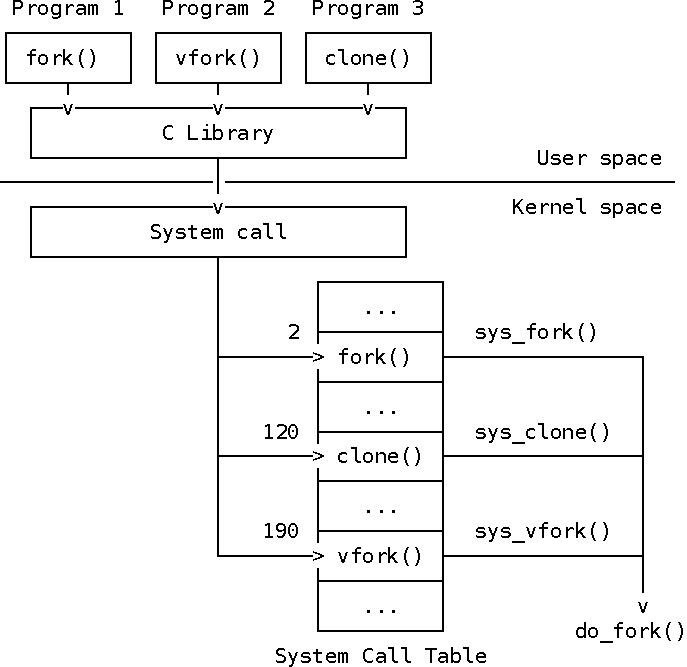
\includegraphics[width=\textwidth]{syscall}
  \end{minipage}
\end{frame}

\begin{frame}{The \texttt{clone()} System Call}
  \begin{center}
    \mode<beamer>{ 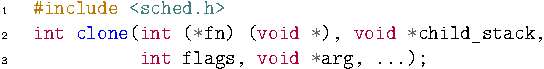
\includegraphics[width=.8\textwidth]{clone-prototype-c} }%
    \mode<article>{ \cfile{figs/pseudo/clone-prototype.c}}
  \end{center}
  \begin{small}
    \begin{description}
    \item[arg 1] the function to be executed, i.e. \texttt{fn(arg)}, which returns an \texttt{int}
    \item[arg 2] a pointer {☛} a (usually malloced) memory space to be used as
      the stack for the new thread
    \item[arg 3] a set of flags used to indicate how much the calling process is to be
      shared. In fact,
      \begin{itemize}
      \item[]  \texttt{clone(0) =\,= fork()}
      \end{itemize}
    \item[arg 4] the arguments passed to the function
    \end{description}
    It returns the PID of the child process or -1 on failure
  \end{small}
  \begin{itemize}
    \item[\$] \texttt{man clone}
  \end{itemize}
\end{frame}

\begin{frame}
  \begin{block}{Some flags:}
    \begin{center}
      \begin{tblr}{colspec={ll}, row{1}={font=\bfseries,c}, cell{2-Z}{1}={font=\ttfamily},%
          hline{1,2,Z},%
        }
        Flag&Shared\\
        CLONE\_FS&File-system info\\
        CLONE\_VM&Same memory space\\
        CLONE\_SIGHAND&Signal handlers\\
        CLONE\_FILES&The set of open files\\
      \end{tblr}
    \end{center}
  \end{block}
  \begin{block}{In practice, one should try to avoid calling \texttt{clone()} directly}
    \begin{itemize}
    \item[] Instead, use a threading library (such as pthreads) which use \texttt{clone()}
      when starting a thread (such as during a call to \texttt{pthread\_create()})
    \end{itemize}
  \end{block}
\end{frame}

\begin{frame}{\texttt{clone()} Example}
  \mode<beamer>{
    \includegraphics[width=.8\textwidth]{clone2}
    \pause 
    \begin{iblock}{Stack grows downwards}
      \includegraphics[width=\textwidth]{child-stack-c}
    \end{iblock}
    \begin{tikzpicture}[remember picture, overlay]
      \node [anchor=east,xshift=-8em,yshift=3em,rotate=-20,scale=6,text opacity=0.6,color=red] at
      (current page.east) {\symbola ✘};
      \node at (current page.south east)
      [anchor=east,xshift=-3em,yshift=3em,scale=8,text opacity=0.6,color=Green] {\symbola ✔};
    \end{tikzpicture}}%
  \mode<article>{ \cfile{../src/proc/clone.c}}
\end{frame}

% \begin{frame}{Stack Grows Downwards}
%   \begin{center}
%     \mode<beamer>{ \includegraphics[width=\textwidth]{child-stack-c} }%
%     \mode<article>{ \cfile{figs/pseudo/child-stack.c} }
%   \end{center}
%   \mode<beamer>{
%     \begin{tikzpicture}[remember picture, overlay]
%       \node [yshift=-0.1em,xshift=9em,rotate=0,scale=12,text opacity=0.7,color=red] at
%       (current page.center) {\symbola ✔}};
%     \end{tikzpicture}}
% \end{frame}

\begin{frame}\mode<beamer>{\frametitle{References}}
  \begin{refsection}
    \nocite{wiki:process, wiki:thread, wiki:pcb}
    \printbibliography[heading=none]
  \end{refsection}
\end{frame}

\lecture[ipc]{ipc}{ipc}

\section{Process Synchronization}
\label{sec:proc-synchr}

\subsection{IPC}
\label{sec:ipc}

\begin{frame}{Interprocess Communication}
  \begin{block}{Example:}
    \begin{itemize}
    \item[\$] \cmd{unicode skull | head -1 | cut -f1 -d' ' | sm -}
    \end{itemize}
  \end{block}
  \begin{block}{IPC issues:}
    \begin{enumerate}
    \item How one process can pass information to another
    \item Be sure processes do not get into each other's way
      \begin{itemize}
      \item[e.g.] in an airline reservation system, two processes compete for the last
        seat
      \end{itemize}
    \item Proper sequencing when dependencies are present
      \begin{itemize}
      \item[e.g.] if A produces data and B prints them, B has to wait until A has produced
        some data
      \end{itemize}
    \end{enumerate}
  \end{block}
  \begin{block}{Two models of IPC:}
    \begin{itemize}
    \item Shared memory
    \item Message passing (e.g. sockets)
    \end{itemize}
  \end{block}
\end{frame}

\begin{frame}{Producer-Consumer Problem}
  \centering
  \mode<beamer>{ 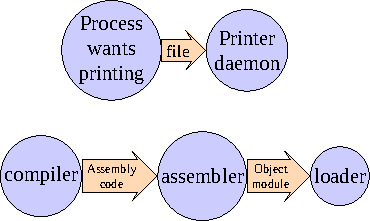
\includegraphics[width=.9\textwidth]{ipc} }
  \mode<article>{ 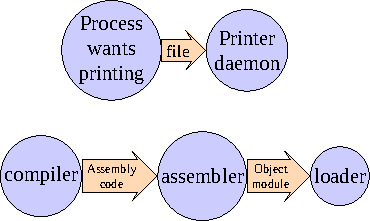
\includegraphics[width=.4\textwidth]{ipc} }
\end{frame}

\subsection{Shared Memory}
\label{sec:shared-memory}

\begin{frame}{Process Synchronization}{Producer-Consumer Problem}
  \begin{itemize}
  \item Consumers don't try to remove objects from Buffer when it is empty.
  \item Producers don't try to add objects to the Buffer when it is full.
  \end{itemize}
  \begin{center}
    \mode<beamer>{ \includegraphics[width=\textwidth]{producer-consumer} }%
    \mode<article>{ \includegraphics[width=.5\textwidth]{producer-consumer-bw} }
  \end{center}
  \begin{center}
    How to define \alert{full/empty}?
  \end{center}
\end{frame}

\begin{frame}{Producer-Consumer Problem}{--- Bounded-Buffer Problem (Circular Array)}
  \begin{minipage}{.5\linewidth}
  \begin{description}
  \item[Front(out):] the first full position
  \item[Rear(in):] the next free position
  \end{description}
  \end{minipage}\quad
  \begin{minipage}{.45\linewidth}
    \mode<beamer>{ 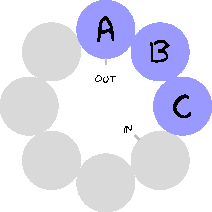
\includegraphics[width=\textwidth]{circular} }%
    \mode<article>{ 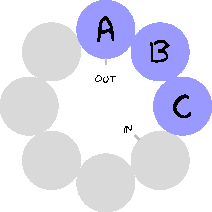
\includegraphics[width=.7\textwidth]{circular} }
  \end{minipage}
  
  Full or empty when ``$front == rear$''?
\end{frame}

\begin{frame}{Producer-Consumer Problem}
  \begin{block}{Common solution:}
    \begin{description}
    \item[Full:] when ``$\mathtt{(in+1)\%BUFFER\_SIZE == out}$''
      \begin{itemize}
      \item[] Actually, this is ``$\mathtt{full - 1}$''
      \end{itemize}
    \item[Empty:] when ``$\mathtt{in == out}$''
    \end{description}
    Can only use ``$\mathtt{BUFFER\_SIZE-1}$'' elements
  \end{block}
  
  \begin{block}{Shared data:}
    \begin{center}
      \mode<beamer>{ \includegraphics[width=.7\textwidth]{shared-data-c} }%
      \mode<article>{ \cfile{figs/pseudo/shared-data.c} }
    \end{center}
  \end{block}
\end{frame}

\begin{frame}{Bounded-Buffer Problem}
  \begin{minipage}{.5\linewidth}
    \begin{block}{Producer:}
      \begin{center}
        \mode<beamer>{ \includegraphics[width=\textwidth]{bounded-buffer-1-c} }%
        \mode<article>{ \cfile{figs/pseudo/bounded-buffer-1.c} }
      \end{center}
    \end{block}
    \begin{block}{Consumer:}
      \begin{center}
        \mode<beamer>{ 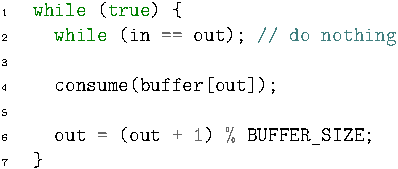
\includegraphics[width=\textwidth]{bounded-buffer-2-c} }%
        \mode<article>{ \cfile{figs/pseudo/bounded-buffer-2.c} }
      \end{center}
    \end{block}
  \end{minipage}\qquad
  \begin{minipage}{.4\linewidth}
    \begin{center}
      \mode<beamer>{ 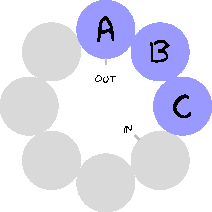
\includegraphics[width=\textwidth]{circular} }%
      \mode<article>{ \includegraphics[width=\textwidth]{circular} }
    \end{center}
  \end{minipage}
\end{frame}

\subsubsection{Pipes and FIFOs}
\label{sec:pipes-fifos}

\begin{itemize}
\item \citetitle[chap.~44]{kerrisk:2010:lpi:1869911}
\end{itemize}

\begin{frame}{Pipe}
  \begin{itemize}
  \item[\$] \cmd{ls | wc -l}
  \end{itemize}
  \begin{center}
    \mode<beamer>{ \includegraphics[width=.75\textwidth]{pipe-ls-wc} }%
    \mode<article>{ \includegraphics[width=.6\textwidth]{pipe-ls-wc} }
  \end{center}
  \begin{itemize}
  \item A pipe is a byte stream
  \item Unidirectional
  \item \texttt{read()} would be blocked if nothing written at the other end
  \end{itemize}
  \ttfamily
  \begin{block}{tee}
    \begin{center}
      \begin{minipage}{.3\linewidth}
        \begin{itemize}
        \item[\$] ls | tee ls.out
        \end{itemize}
      \end{minipage}\quad
      \begin{minipage}{.4\linewidth}
        \mode<beamer>{ \includegraphics[width=\textwidth]{tee} }%
        \mode<article>{ \includegraphics[width=.6\textwidth]{tee} }
      \end{minipage}
    \end{center}
  \end{block}
\end{frame}

\begin{itemize}
\item When we say that a pipe is a byte stream, we mean that there is no concept of
  messages or message boundaries when using a pipe. The process reading from a pipe can
  read blocks of data of any size, regardless of the size of blocks written by the writing
  process. Furthermore, the data passes through the pipe sequentially --- bytes are read from
  a pipe in exactly the order they were written. It is not possible to randomly access the
  data in a pipe using \texttt{lseek()}. \citetitle[chap.~44]{kerrisk:2010:lpi:1869911}
\end{itemize}


\begin{frame}
\begin{center}
  \mode<beamer>{ \includegraphics[width=.6\textwidth]{pipe} }%
  \mode<article>{ \includegraphics[width=.4\textwidth]{pipe} }
\end{center}
\begin{itemize}
\item No direct link between A and B (need system calls)
\item A pipe is simply a buffer maintained in kernel memory
  \begin{itemize}
  \item[\$] \cmd{cat /proc/sys/fs/pipe-max-size}
  \end{itemize}
\end{itemize}
\end{frame}

\begin{frame}{\texttt{pipe()}}
  \begin{center}
    \begin{minipage}{.3\linewidth}
      \mode<beamer>{ \includegraphics[width=\textwidth]{pipe-prototype-c} }%
      \mode<article>{\cfile{../src/proc/pipe-prototype.c}}
    \end{minipage}\quad
    \begin{minipage}{.3\linewidth}
      \mode<beamer>{ \includegraphics[width=\textwidth]{pipe1} }%
      \mode<article>{ \includegraphics[width=.8\textwidth]{pipe1} }
    \end{minipage}
  \end{center}
  \begin{description}
  \item[\texttt{pipe()} + \texttt{fork()}]
  \end{description}
  \begin{center}
    \mode<beamer>{ \includegraphics[width=.6\textwidth]{pipe2} }%
    \mode<article>{ \includegraphics[width=.5\textwidth]{pipe2} }
  \end{center}
\end{frame}

\begin{itemize}
\item Pipes must have a reader and a writer. If a process tries to write to a pipe that
  has no reader, it will be sent the SIGPIPE signal from the kernel. This is imperative
  when more than two processes are involved in a
  pipeline. (\url{http://www.tldp.org/LDP/lpg/node20.html})
\item While it is possible for the parent and child to both read from and write to the
  pipe, this is not usual. Therefore, immediately after the \texttt{fork()}, one process
  closes its descriptor for the write end of the pipe, and the other closes its descriptor
  for the read end. For example, if the parent is to send data to the child, then it would
  close its read descriptor for the pipe, \texttt{filedes[0]}, while the child would close
  its write descriptor for the pipe, \texttt{filedes[1]}.
  
  One reason that it is not usual to have both the parent and child reading from a single
  pipe is that if two processes try to simultaneously read from a pipe, we can't be sure
  which process will be the first to succeed—the two processes race for data.  Preventing
  such races would require the use of some synchronization mechanism.  However, if we
  require bidirectional communication, there is a simpler way: just create two pipes, one
  for sending data in each direction between the two processes.  (If employing this
  technique, then we need to be wary of deadlocks that may occur if both processes block
  while trying to read from empty pipes or while trying to write to pipes that are already
  full.) \citetitle[chap.~44, p.~893]{kerrisk:2010:lpi:1869911}
\item Pipes can be used for communication between any two (or more) related processes, as
  long as the pipe was created by a common ancestor before the series of \texttt{fork()}
  calls that led to the existence of the processes. For example, a pipe could be used for
  communication between a process and its grandchild. The first process creates the pipe,
  and then forks a child that in turn forks to yield the grandchild. A common scenario is
  that a pipe is used for communication between two siblings --- their parent creates the
  pipe, and then creates the two children. This is what the shell does when building a
  pipeline.
\item \textbf{Closing unused pipe file descriptors}. The process reading from the pipe
  closes its write descriptor for the pipe, so that, when the other process completes its
  output and closes its write descriptor, the reader sees end-of-file (once it has read
  any outstanding data in the pipe).  If the reading process doesn't close the write end
  of the pipe, then, after the other process closes its write descriptor, the reader won't
  see end-of-file, even after it has read all data from the pipe. Instead, a
  \texttt{read()} would block waiting for data, because the kernel knows that there is
  still at least one write descriptor open for the pipe. That this descriptor is held open
  by the reading process itself is irrelevant; in theory, that process could still write
  to the pipe, even if it is blocked trying to read.  For example, the \texttt{read()}
  might be interrupted by a signal handler that writes data to the pipe.

  The writing process closes its read descriptor for the pipe for a different reason.
  When a process tries to write to a pipe for which no process has an open read
  descriptor, the kernel sends the SIGPIPE signal to the writing process. By default, this
  signal kills a process. A process can instead arrange to catch or ignore this signal, in
  which case the \texttt{write()} on the pipe fails with the error EPIPE (broken
  pipe). Receiving the SIGPIPE signal or getting the EPIPE error is a useful indication
  about the status of the pipe, and this is why unused read descriptors for the pipe
  should be closed.

  If the writing process doesn't close the read end of the pipe, then, even after the
  other process closes the read end of the pipe, the writing process will still be able to
  write to the pipe. Eventually, the writing process will fill the pipe, and a further
  attempt to write will block indefinitely.

  One final reason for closing unused file descriptors is that it is only after all file
  descriptors in all processes that refer to a pipe are closed that the pipe is destroyed
  and its resources released for reuse by other processes. At this point, any unread data
  in the pipe is lost.
\end{itemize}

\begin{frame}
  \mode<beamer>{ \includegraphics[height=\textheight]{simple_pipe-c} }%
  \mode<article>{\cfile{../src/proc/simple_pipe.c}}
\end{frame}

\begin{itemize}
\item
  \url{https://stackoverflow.com/questions/5422831/what-is-the-difference-between-using-exit-exit-in-a-conventional-linux-fo}
\item \texttt{\_exit(2)}
\end{itemize}

\begin{frame}{Named Pipe (FIFO)}
  \begin{description}
  \item[PIPEs] pass data between related processes.
  \item[FIFOs] pass data between any processes.
  \end{description}
  \begin{block}{\texttt{mkfifo}}
    \begin{center}
      \begin{minipage}{.45\linewidth}\ttfamily
        \begin{itemize}
        \item[\$] mkfifo myfifo
        \item[\$] echo hello > myfifo
        \item[\$] cat myfifo
        \end{itemize}
      \end{minipage}\quad
      \begin{minipage}{.5\linewidth}
        \mode<beamer>{ \includegraphics[width=\textwidth]{fifo} }%
        \mode<article>{ \includegraphics[width=.6\textwidth]{fifo} }
      \end{minipage}
    \end{center}
  \end{block}
  \ttfamily
  \begin{block}{tee}
    \begin{minipage}{.5\linewidth}
      \begin{itemize}
      \item[\$] echo hello | tee myfifo
      \item[\$] wc myfifo
      \end{itemize}
    \end{minipage}\quad
    \begin{minipage}{.45\linewidth}
      \mode<beamer>{ \includegraphics[width=\textwidth]{fifo-tee} }%
      \mode<article>{ \includegraphics[width=.6\textwidth]{fifo-tee} }
    \end{minipage}
  \end{block}
\end{frame}

\begin{itemize}
\item \url{https://en.wikipedia.org/wiki/Named_pipe}
\end{itemize}

\begin{frame}{IPC With FIFO}
  \mode<beamer>{ \includegraphics[height=.9\textheight]{fifo2-c} }%
  \mode<article>{\cfile{../src/proc/fifo2.c}}
\end{frame}

% \begin{frame}{}{}
%   {\ttfamily
%     \begin{itemize}
%     \item[\$] watch -n.1 'lsof /tmp/myfifo'
%     \item[\$] ./a.out O\_RDONLY
%     \item[\$] ./a.out O\_WRONLY
%     % \item[\$] ./a.out O\_RDONLY O\_NONBLOCK
%     % \item[\$] ./a.out O\_WRONLY O\_NONBLOCK
%     \end{itemize}}
%   % \begin{block}{\texttt{O\_NONBLOCK}}
%   %   \begin{itemize}
%   %   \item A \texttt{read()/write()} will wait on an empty blocking FIFO
%   %   \item A \texttt{read()} on an empty nonblocking FIFO will return 0 bytes
%   %   \item \cmd{open(const char *path, O\_WRONLY | O\_NONBLOCK);}
%   %     \begin{itemize}
%   %     \item Returns an error (-1) if FIFO not open
%   %     \item Okay if someone's reading the FIFO
%   %     \end{itemize}
%   %   \item If opened with \texttt{O\_RDWR}, the result is undefined.  \mode<article>{If you
%   %       do want to pass data in both directions, it's much better to use a pair of FIFOs
%   %       or pipes, one for each direction.}
%   %   \end{itemize}
%   % \end{block}
% \end{frame}

\begin{itemize}
%\item If opened with \texttt{O\_RDWR}, the result is undefined. 
\item There are four legal combinations of \texttt{O\_RDONLY}, \texttt{O\_WRONLY}, and the
  \texttt{O\_NONBLOCK} flag. 
\end{itemize}
\begin{longlisting}
  \cfile{../src/proc/o_nonblock.c}
\end{longlisting}

\subsubsection{Message Queues}
\label{sec:message-queues}

\begin{frame}{Message Queues}
  \centering
  \begin{minipage}{.25\linewidth}
    \mode<beamer>{ \includegraphics[width=\textwidth]{mq} }%
    \mode<article>{ \includegraphics[width=.6\textwidth]{mq} }
  \end{minipage}\qquad
  \begin{minipage}{.4\linewidth}
    \mode<beamer>{ \includegraphics[width=\textwidth]{circular} }%
    \mode<article>{ \includegraphics[width=.6\textwidth]{circular} }
  \end{minipage}
\end{frame}

\begin{itemize}
\item \citetitle[Sec.~52.3]{kerrisk:2010:lpi:1869911}
\item \texttt{mq\_overview(7)}
\item \texttt{sem\_overview(7)}
\item \texttt{shm\_overview(7)}
\item \url{https://www.uninformativ.de/blog/postings/2016-05-16/0/POSTING-en.html}
\end{itemize}

\begin{frame}{Message Queues}{Send}
\begin{center}
  \mode<beamer>{ \includegraphics[width=\textwidth]{mq-send} }%
  \mode<article>{\cfile{../src/proc/mq-send.c}}
\end{center}
\end{frame}

\begin{frame}{Message Queues}{Receive}
  \centering
  \mode<beamer>{ \includegraphics[height=.85\textheight]{mq-recv} }%
  \mode<article>{\cfile{../src/proc/mq-recv.c}}
\end{frame}

\begin{frame}<article>{Relationship Between Kernel Data Structures}
\begin{center}
  \mode<beamer>{ \includegraphics[width=.8\textwidth]{msgq} }%
  \mode<article>{ \includegraphics[width=.6\textwidth]{msgq} }
\end{center}
\end{frame}

\subsection{Race Condition and Mutual Exclusion}
\label{sec:race-condition}

\begin{frame}{Race Conditions}
  \begin{block}{Now, let's have two producers}
    \centering
    \mode<beamer>{ \includegraphics[width=.7\textwidth]{mos-figs-2-18} }%
    \mode<article>{ \includegraphics[width=.45\textwidth]{mos-figs-2-18} }
  \end{block}
\end{frame}

\begin{frame}{Race Conditions}{Two producers}
  \begin{center}
    \mode<beamer>{ \includegraphics[width=.4\textwidth]{two-producer-c} }%
    \mode<article>{ \cfile{figs/pseudo/two-producer.c} }
  \end{center}
  \begin{block}{Process A and B do the same thing:}
    \begin{center}
      \mode<beamer>{ \includegraphics[width=.7\textwidth]{two-producer-2-c} }%
      \mode<article>{ \cfile{figs/pseudo/two-producer-2.c} }
    \end{center}
  \end{block}
\end{frame}

\begin{frame}{Race Conditions}
  \begin{description}
  \item[Problem:] Process \texttt{B} started using one of the \emph{shared variables} before
    Process \texttt{A} was finished with it.
  \item[Solution:] \alert{Mutual exclusion}. If one process is using a shared variable or
    file, the other processes will be excluded from doing the same thing.
  \end{description}
\end{frame}

\begin{frame}{Critical Regions}{Mutual Exclusion}
  \begin{description}
  \item[Critical Region:] is a piece of code accessing a common resource.
  \end{description}
  \begin{center}
    \mode<beamer>{ \includegraphics[width=\textwidth]{mos-figs-2-19} }%
    \mode<article>{ \includegraphics[width=.7\textwidth]{mos-figs-2-19} }
  \end{center}
\end{frame}

\begin{frame}[label=cond]{Critical Region}
  A solution to the critical region problem must satisfy three conditions:
  \begin{description}
  \item[Mutual Exclusion:] No two process may be simultaneously inside their critical regions.
  \item[Progress:] No process running outside its critical region may block other processes.
  \item[Bounded Waiting:] No process should have to wait forever to enter its critical region.
  \end{description}
\end{frame}

\begin{frame}{Mutual Exclusion With Busy Waiting}{Disabling Interrupts}
  \begin{minipage}{.3\linewidth}
    \mode<beamer>{ \includegraphics[width=\textwidth]{disable-int-c} }%
    \mode<article>{ \cfile{figs/pseudo/disable-int.c} }
  \end{minipage}\quad
  \begin{minipage}{.65\linewidth}
    \begin{block}{Problems:}
      \begin{itemize}
      \item It's not wise to give user process the power of turning off INTs.
        \begin{itemize}
        \item Suppose one did it, and never turned them on again
        \end{itemize}
      \item useless for multiprocessor system
      \end{itemize}
    \end{block}
  \end{minipage}\\[1em]
  Disabling INTs is often a useful technique within the kernel itself but is not a general
  mutual exclusion mechanism for user processes.
\end{frame}

\begin{frame}{Mutual Exclusion With Busy Waiting}{Lock Variables}
  \begin{minipage}{.45\linewidth}
    \mode<beamer>{ \includegraphics[width=\textwidth]{lock-var-c} }%
    \mode<article>{ \cfile{figs/pseudo/lock-var.c} }
  \end{minipage}\quad
  \begin{minipage}{.5\linewidth}
    \begin{block}{Problem:}
      \begin{itemize}
      \item What if an interrupt occurs right at line 5?
      \item Checking the lock again while backing from an interrupt?
      \end{itemize}
    \end{block}
  \end{minipage}
\end{frame}

\begin{frame}{Mutual Exclusion With Busy Waiting}{Strict Alternation}
  \begin{center}
    \mode<beamer>{ \includegraphics[width=\textwidth]{strict-alternation} }%
    \mode<article>{ \includegraphics[width=.5\textwidth]{strict-alternation-bw} }
  \end{center}
  \begin{block}{Problem: violates \hyperlink{cond}{condition-2}}
    \begin{itemize}
    \item One process can be blocked by another not in its critical region.
    \item Requires the two processes strictly alternate in entering their critical region.
    \end{itemize}
  \end{block}
\end{frame}

\begin{frame}{Mutual Exclusion With Busy Waiting}{Peterson's Solution}
  \begin{center}
    \mode<beamer>{ \includegraphics[width=.8\textwidth]{peterson} }%
    \mode<article>{ \includegraphics[width=.6\textwidth]{peterson-bw} }
  \end{center}
  \begin{refsection}
    \nocite{wiki:peterson}
    \printbibliography[heading=none]
  \end{refsection}
\end{frame}

\begin{frame}{Mutual Exclusion With Busy Waiting}{Lock file}
  \mode<beamer>{ \includegraphics[width=\textwidth]{lock2-c} }%
  \mode<article>{\cfile{../src/proc/lock2.c}}
  \begin{itemize}
  \item[☹] Lock file could be left in system after \LKeyCtrlX{c}
  \end{itemize}
\end{frame}

\begin{frame}
  \mode<beamer>{ \includegraphics[width=\textwidth]{lock2-sigint-c} }%
  \mode<article>{\cfile{../src/proc/lock2-sigint.c}}
  \begin{itemize}
  \item[☹] \texttt{sigint()} is too crude to be reliable. Need a more sophisticated design.
  \end{itemize}
\end{frame}

\begin{frame}{Mutual Exclusion With Busy Waiting}{Hardware Solution: The TSL Instruction}
  \begin{block}{Lock the memory bus}
    \begin{center}
      \mode<beamer>{ \includegraphics[width=\textwidth]{mos-figs-2-22} }%
      \mode<article>{ \includegraphics[width=.6\textwidth]{mos-figs-2-22} }
    \end{center}
  \end{block}
\end{frame}

See also: \citetitle[Sec.~2.3.3, \emph{Mutual Exclusion With Busy Waiting},
p.~124]{tanenbaum2015modern}.

\begin{frame}{Mutual Exclusion Without Busy Waiting}{Sleep \& Wakeup}
  \begin{center}
    \mode<beamer>{ \includegraphics[width=.8\textwidth]{sleep-wakeup}\pause%
      \begin{tikzpicture}[remember picture, overlay]
        \node [rotate=10,scale=5,text opacity=0.5,color=red] at (current page.center)
        {Deadlock!};
      \end{tikzpicture}}%
    \mode<article>{ \includegraphics[width=.6\textwidth]{sleep-wakeup-bw-crop} }
  \end{center}
\end{frame}

\begin{frame}{Producer-Consumer Problem}{Race Condition}
  \begin{block}{Problem}
    \begin{enumerate}
    \item Consumer is going to sleep upon seeing an empty buffer, but INT occurs;
    \item Producer inserts an item, increasing \texttt{count} to \texttt{1}, then call
      \texttt{wakeup(consumer)};
    \item But the consumer is not asleep, though \texttt{count} was \texttt{0}. So \emph{the
        \texttt{wakeup()} signal is lost};
    \item Consumer is back from INT remembering \texttt{count} is \texttt{0}, and goes to
      sleep;
    \item Producer sooner or later will fill up the buffer and also goes to sleep;
    \item Both will sleep forever, and waiting to be waken up by the other
      process. Deadlock!
    \end{enumerate}
  \end{block}
\end{frame}

\begin{frame}{Producer-Consumer Problem}{Race Condition}
  \begin{block}{Solution: Add a \emph{wakeup waiting bit}}
    \begin{enumerate}
    \item The bit is set, when a wakeup is sent to an awaken process;
    \item Later, when the process wants to sleep, it checks the bit first. Turns it off if it's set,
      and stays awake.
    \end{enumerate}
    What if many processes try going to sleep?
  \end{block}
\end{frame}

\subsection{Semaphores}
\label{sec:semaphores}

\begin{frame}[fragile,squeeze]{What is a Semaphore?\,\includegraphics[width=1em]{semaphore-papa}}
  \begin{itemize}
  \item A locking mechanism
  \item An integer or ADT\\[1em]
  \end{itemize}
  \begin{minipage}{.42\linewidth}
    \begin{small}
      \begin{tblr}{colspec={ll},cell{1}{1}={c=2}{c,font=\bfseries},hline{1,2,Z},
          row{2-Z}={font=\ttfamily},
        }
        Atomic Operations\\
        P()         &V()\\
        Wait()      &Signal()\\
        Down()      &Up()\\
        Decrement() &Increment()\\
        \ldots      &\ldots\\
      \end{tblr}
    \end{small}
  \end{minipage}\quad
  \begin{minipage}{.53\linewidth}
    \mode<beamer>{ \includegraphics[width=\textwidth]{down-up} }%
    \mode<article>{ \includegraphics[width=\textwidth]{down-up-bw} }
  \end{minipage}
  \begin{block}{More meaningful names:}
    \begin{itemize}
    \item \texttt{increment\_and\_wake\_a\_waiting\_process\_if\_any()}
    \item \texttt{decrement\_and\_block\_if\_the\_result\_is\_negative()}
    \end{itemize}
  \end{block}
\end{frame}

\begin{frame}{Semaphore\,\includegraphics[width=1em]{semaphore-papa}}%{P/V, Down/Up, Wait/Signal...}
\begin{block}{How to ensure atomic?}
  \begin{enumerate}
  \item For single CPU, implement \texttt{up()} and \texttt{down()} as system calls, with the
    OS disabling all interrupts while accessing the semaphore;
  \item For multiple CPUs, to make sure only one CPU at a time examines the semaphore, a lock
    variable should be used with the TSL instructions.
  \end{enumerate}
\end{block}
\end{frame}

\begin{frame}{Semaphore is a Special Integer\,\includegraphics[width=1em]{semaphore-papa}}
  \begin{block}{A semaphore is like an integer, with three differences:}
    \begin{enumerate}
    \item You can initialize its value to any integer, but after that the only operations
      you are allowed to perform are \emph{increment} (\texttt{S++}) and \emph{decrement}
      (\texttt{S-\,-}).
    \item When a thread decrements the semaphore, if the result is negative (S ⩽ 0), the
      thread blocks itself and cannot continue until another thread increments the
      semaphore.
    \item When a thread increments the semaphore, if there are other threads waiting, one
      of the waiting threads gets unblocked.
    \end{enumerate}
  \end{block}
\end{frame}

\begin{frame}{Why Semaphores?\,\includegraphics[width=1em]{semaphore-papa}}
  We don't need semaphores to solve synchronization problems, but there are some advantages to using
  them:
  \begin{itemize}
  \item Semaphores impose deliberate constraints that help programmers avoid errors.
  \item Solutions using semaphores are often clean and organized, making it easy to demonstrate
    their correctness.
  \item Semaphores can be implemented efficiently on many systems, so solutions that use semaphores
    are portable and usually efficient.
  \end{itemize}
\end{frame}

\begin{frame}{The Simplest Use of Semaphore}{Signaling}
  \begin{itemize}
  \item One thread sends a signal to another thread to indicate that something has
    happened
  \item it solves the serialization problem
    \begin{itemize}
    \item[] Signaling makes it possible to guarantee that a section of code in one thread
      will run before a section of code in another thread
    \end{itemize}
  \end{itemize}
  \begin{center}
    \mode<beamer>{ \includegraphics[width=.7\textwidth]{sem-signaling} }%
    \mode<article>{ \includegraphics[width=.4\textwidth]{sem-signaling} }
  \end{center}
  \begin{center}
    What's the initial value of \texttt{sem}?
  \end{center}
\end{frame}

\begin{frame}{Semaphore}{Rendezvous Puzzle}
  \begin{center}
    \mode<beamer>{ \includegraphics[width=.8\textwidth]{rendezvous} }%
    \mode<article>{ \includegraphics[width=.4\textwidth]{rendezvous} }
  \end{center}
  \begin{itemize}
  \item[Q:] How to guarantee that
    \begin{enumerate}
    \item \texttt{a1} happens before \texttt{b2}, and
    \item \texttt{b1} happens before \texttt{a2}
    \end{enumerate}
    \texttt{a1} $\rightarrow{}$ \texttt{b2};\quad \texttt{b1} $\rightarrow{}$ \texttt{a2}
  \item[Hint:] Use two semaphores initialized to 0.
  \end{itemize}
\end{frame}

\begin{frame}[fragile]
  \begin{center}
    \begin{tblr}{colspec={lll},hlines,row{1}={c,font=\bfseries},
      cell{2,3,4}{2,3}={font=\ttfamily}}
      &\textbf{Thread A:}&\textbf{Thread B:}\\
      Solution 1:&%
      \begin{tblr}{l}
        {statement a1\\sem1.wait()\\sem2.signal()\\statement a2}\\
      \end{tblr} &%
      \begin{tblr}{l}
        {statement b1\\sem1.signal()\\sem2.wait()\\statement b2}\\
      \end{tblr}\\
      Solution 2:&%
      \begin{tblr}{l}
        {statement a1\\sem2.signal()\\sem1.wait()\\statement a2}\\
      \end{tblr} &%
      \begin{tblr}{l}
        {statement b1\\sem1.signal()\\sem2.wait()\\statement b2}\\
      \end{tblr} \\
      Solution 3:&%
      \begin{tblr}{l}
        {statement a1\\sem2.wait()\\sem1.signal()\\statement a2}\\
      \end{tblr} &%
      \begin{tblr}{l}
        {statement b1\\sem1.wait()\\sem2.signal()\\statement b2}\\
      \end{tblr}\\
    \end{tblr}
  \end{center}
  \mode<beamer>{\pause
    \begin{tikzpicture}[remember picture, overlay]
      \node [rotate=10,scale=3,opacity=0.5,color=red,anchor=south,%
      yshift=2.3ex,xshift=2ex] at (current page.south) {Deadlock!};
    \end{tikzpicture}
  } \mode<article>{ \alert{Solution 3 has deadlock!}  }
\end{frame}

\begin{frame}{Example: Signaling With Semaphore}% 
  \centering
  \mode<beamer>{ \includegraphics[width=.55\textwidth]{thread-semaphore} }%
  \mode<article>{\cfile{../src/proc/thread-semaphore.c}}
\end{frame}

\begin{itemize}
\item \citetitle[Sec.~12.5]{matthew2008beginning}
\item \url{https://stackoverflow.com/questions/368322/differences-between-system-v-and-posix-semaphores}
\end{itemize}

\begin{frame}
  \begin{block}{Mutex}
    \begin{itemize}
    \item A second common use for semaphores is to enforce \underline{mut}ual
      \underline{ex}clusion
    \item It guarantees that only one thread accesses the shared variable at a time
    \item A \texttt{mutex} is like a token that passes from one thread to another, allowing
      one thread at a time to proceed
    \end{itemize}
  \end{block}
  \begin{itemize}
  \item[Q:] Add semaphores to the following example to enforce mutual exclusion to the
    shared variable \texttt{i}.
  \end{itemize}
  \begin{multicols}{2}
    \begin{description}
    \item[Thread A:] \cfbox{violet}{\texttt{i++}}
    \item[Thread B:] \cfbox{violet}{\texttt{i++}}
    \end{description}
  \end{multicols}
  \begin{description}
  \item[Why?] Because \texttt{i++} is not atomic.
  \end{description}
\end{frame}

\begin{frame}{\texttt{i++} {\small can go wrong!}}
  \mode<beamer>{\centering\includegraphics[height=.9\textheight]{atomic-non} }%
  \mode<article>{\cfile{../src/proc/atomic-non.c}}
\end{frame}

\begin{frame}%{\texttt{i++} is Not Thread Safe}
  \begin{block}{\texttt{i++} is not atomic in assembly language}
    \begin{center}
      \mode<beamer>{ \includegraphics[width=.8\textwidth]{ipp} }%
      \mode<article>{ \includegraphics[width=.5\textwidth]{ipp-bw} }
    \end{center}
  \end{block}
  Interrupts might occur in between. So, \texttt{i++} needs to be protected with a \texttt{mutex}.
\end{frame}


\begin{frame}{Mutex Solution}
  \begin{block}{Create a semaphore named \texttt{mutex} that is initialized to
      \texttt{1}}
    \begin{itemize}
    \item[1:] a thread may proceed and access the shared variable
    \item[0:] it has to wait for another thread to release the mutex
    \end{itemize}
  \end{block}
  \begin{center}
    \mode<beamer>{ \includegraphics[width=.8\textwidth]{mutex-ipp} }%
    \mode<article>{ \includegraphics[width=.5\textwidth]{mutex-ipp} }
  \end{center}
\end{frame}

\begin{frame}
  \centering
  \mode<beamer>{ \includegraphics[height=\textheight]{atomic-mutex} }%
  \mode<article>{\cfile{../src/proc/atomic-mutex.c}}
\end{frame}

\begin{frame}
\begin{center}
  \mode<beamer>{ \includegraphics[width=.7\textwidth]{mutex} }%
  \mode<article>{\cfile{../src/proc/mutex.c}}
\end{center}
\end{frame}

\begin{frame}[label=comp,fragile]{Multiplex --- Without Busy Waiting}
  \begin{center}
    \mode<beamer>{ \includegraphics[width=.7\textwidth]{sem-multiplex} }
    \mode<article>{ \includegraphics[width=.5\textwidth]{sem-multiplex-bw} }
  \end{center}
  \vskip -1ex
  {\ttfamily\footnotesize
    \begin{itemize}
    \item[if] S.space < 0,\\
      S.space == Number of queuing producers
    \item[if] S.space > 5,\\
      S.space == Number of queuing consumers + 5
    \end{itemize}}
\end{frame}

\paragraph{The work flow}

There are several processes running simultaneously. They all need to
access some common resources.
\begin{enumerate}
\item Assuming \texttt{S.space == 3} in the beginning
\item Process P1 comes and take one resource away. \texttt{S.space == 2} now.
\item Process P2 comes and take the 2nd resource away. \texttt{S.space == 1} now.
\item Process P3 comes and take the last resource away. \texttt{S.space == 0} now.
\item Process P4 comes and sees nothing left. It has to sleep. \texttt{S.space == -1} now.
\item Process P5 comes and sees nothing left. It has to sleep. \texttt{S.space == -2} now.
\item At this moment, there are 2 processes (P4 and P5) sleeping. In another word, they
  are queuing for resources.
\item Now, P1 finishes using the resource, and released it. After it does a
  \texttt{S.space++}, it finds out that \texttt{S.space <= 0}. So it wakes up a Process
  (say P4) in the queue.
\item P4 wakes up, and back to execute the instruction right after \texttt{sleep()}.
\item P4 (or P2|P3) finishes using the resource, and releases it. After it does a
  \texttt{S.space++}, it finds out that \texttt{S.space <= 0}. So it wakes up P5 in the
  queue.
\item the queue is empty now.
\end{enumerate}

\begin{frame}{Barrier}
  % the little book of semaphores
  \begin{center}
    \mode<beamer>{ \includegraphics[width=.65\textwidth]{barrier} }%
    \mode<article>{ \includegraphics[width=.6\textwidth]{barrier} }
  \end{center}
  \begin{enumerate}
  \item Processes approaching a barrier
  \item All processes but one blocked at the barrier
  \item When the last process arrives at the barrier, all of them are let through
  \end{enumerate}
  \begin{minipage}{.7\linewidth}
    \begin{block}{Synchronization requirement:}
      No thread executes \texttt{critical\_point()} until after all threads have executed
      \texttt{specific\_task()}.
    \end{block}
  \end{minipage}\quad
  \begin{minipage}{.25\linewidth}
    \begin{tblr}{colspec={l},rows={font=\ttfamily}}
      {specific\_task()\\critical\_point()}
    \end{tblr}
  \end{minipage}
\end{frame}

\begin{frame}{Barrier Solution}
  \begin{minipage}{.4\linewidth}
    \mode<beamer>{ \includegraphics[width=\textwidth]{barrier-1-py} }%
    \mode<article>{ \pyfile{figs/pseudo/barrier-1.py} }
  \end{minipage}
  \begin{minipage}{.57\linewidth}
    {\footnotesize
      \begin{description}
      \item[count:] keeps track of how many threads have arrived
      \item[mutex:] provides exclusive access to \texttt{count}
      \item[barrier:] is locked ($\le 0$) until all threads arrive%; then it should be
        % unlocked ($\ge 1$)
      \item[When \texttt{barrier.value<0},]\,\\ \texttt{barrier.value == Number of queueing processes}
      \end{description}
    }
  \end{minipage}
  \begin{center}
    \mode<beamer>{ \includegraphics[width=.78\textwidth]{barrier-2} }%
    \mode<article>{ \includegraphics[width=.5\textwidth]{barrier-2-bw} }
  \end{center}
  \pause
  \begin{center}
    \alert{Only one thread can pass the barrier!}
  \end{center}
  \mode<beamer>{
    \begin{tikzpicture}[remember picture, overlay]
      \node [scale=10,text opacity=0.3,color=red,yshift=-.5em,xshift=-.4em] at (current
      page.center) {\symbola ✔};

      \node [scale=2.2,text opacity=0.3,color=red,yshift=-2em,xshift=3em,rotate=20] at
      (current page.center) {Deadlock!};
    \end{tikzpicture} }
\end{frame}

\begin{frame}{Barrier Solution}
  \begin{center}
    \mode<beamer>{
      \includegraphics[width=\textwidth]{barrier-3}
    } \mode<article>{
      \includegraphics[width=.5\textwidth]{barrier-3-bw}
    }
  \end{center}
  \mode<beamer>{
    \pause
    \begin{center}
      {\color{red}\danger{}} \alert{Blocking on a semaphore while holding a
        mutex!} {\color{red}\danger{}} 
    \end{center}
    \begin{tikzpicture}[remember picture, overlay]
      \node [rotate=40,scale=3.5,text opacity=0.3,color=red,xshift=2.2em,yshift=-1em] at
      (current page.center) {Deadlock!};
    \end{tikzpicture}
  }
  \mode<article>{
    \begin{center}
      \danger{} Blocking on a semaphore while holding a mutex!\danger{}
    \end{center}
  }
\end{frame}

\begin{frame}%{Barrier Solution}
  \begin{center}
    \begin{tblr}{colspec={l},rows={font=\ttfamily}}
      {barrier.wait();\\barrier.signal();}
    \end{tblr}
  \end{center}
  \begin{block}{Turnstile}
    This pattern, a \texttt{wait} and a \texttt{signal} in rapid succession, occurs often
    enough that it has a name called a \emph{turnstile}, because
    \begin{itemize}
    \item it allows one thread to pass at a time, and
    \item it can be locked to bar all threads
    \end{itemize}
  \end{block}
\end{frame}

% \begin{frame}{Semaphores}{Producer-Consumer Problem}
%   \begin{block}{Whenever an event occurs}
%     \begin{itemize}
%     \item a producer thread creates an \emph{event object} and adds it to the event
%       buffer. Concurrently,
%     \item consumer threads take events out of the buffer and process them. In this case,
%       the consumers are called ``\emph{event handlers}''.
%     \end{itemize}
%   \end{block}
%   \begin{center}
%     \mode<beamer>{ \includegraphics[width=.9\textwidth]{event} }%
%     \mode<article>{ \includegraphics[width=.5\textwidth]{event-bw} }
%   \end{center}
%   \begin{itemize}
%   \item[Q:] Add synchronization statements to the producer and consumer code to enforce
%     the synchronization constraints
%     \begin{enumerate}
%     \item Mutual exclusion
%     \item Serialization
%     \end{enumerate}
%   \end{itemize}
% \end{frame}

See also: \citetitle[Sec.~4.1, \emph{Producer-Consumer Problem}]{downey2008semaphores}.

% \begin{frame}{Semaphores --- Producer-Consumer Problem}{Solution}
%   \begin{block}{Initialization:}
%     \begin{center}
%       \begin{tabular}{>{\ttfamily}l}
%         mutex = Semaphore(1)\\
%         items = Semaphore(0)
%       \end{tabular}
%     \end{center}
%     \begin{itemize}
%     \item \texttt{mutex} provides exclusive access to the buffer
%     \item \texttt{items}:
%       \begin{itemize}
%       \item[{\nerd }] number of items in the buffer
%       \item[{\nerd }] number of consumer threads in queue
%       \end{itemize}
%     \end{itemize}
%   \end{block}
% \end{frame}

% \begin{frame}{Semaphores --- Producer-Consumer Problem}{Solution}
%   \begin{center}
%     \mode<beamer>{ \includegraphics[width=\textwidth]{event-2} }%
%     \mode<article>{ \includegraphics[width=.5\textwidth]{event-2-bw} }
%   \end{center}
  
%   \mode<article>{
%     \begin{itemize}
%     \item[\danger{}] any time you wait for a semaphore while holding a mutex!
%     \end{itemize}}
%   \mode<beamer>{\pause    
%     \begin{itemize}
%     \item[{\color{red}\danger{}}] any time you wait for a semaphore while holding a mutex!
%     \end{itemize}
%     \begin{tikzpicture}[remember picture, overlay]
%       \node [rotate=15,scale=2.5,text opacity=0.4,color=red,yshift=-3em,xshift=2.5em] at
%       (current page.center) {Deadlock!};
%     \end{tikzpicture}}
% \end{frame}

% \begin{minipage}{.4\linewidth}
% \begin{ccode}
%   items.signal()
%   {
%     items++;
%     if(items == 0)
%       wakeup(consumer);
%   }  
% \end{ccode} 
% \end{minipage}
% \qquad\qquad
% \begin{minipage}{.4\linewidth}
% \begin{ccode}
%   items.wait()
%   {
%     items--;
%     if(items < 0)
%       sleep();
%   }
% \end{ccode} 
% \end{minipage}

\begin{frame}{Producer-Consumer Problem With Bounded-Buffer}
  \begin{block}{Given:}
    \begin{center}
      \begin{tblr}{colspec={l},rows={font=\ttfamily}}
        {semaphore items = 0;\\semaphore spaces = BUFFER\_SIZE;}
      \end{tblr}
    \end{center}
  \end{block}
  \begin{block}{Can we?}
    \begin{center}
      \begin{tblr}{colspec={l},rows={font=\ttfamily}}
        {if (items >= BUFFER\_SIZE)\\\qquad{}producer.block();}
      \end{tblr}
    \end{center}
    \begin{description}
    \item[if] the buffer is full
    \item[then] the producer blocks until a consumer removes an item
    \end{description}
  \end{block}
  \pause 
  \alert{No!} We can't check the current value of a semaphore, because
  \begin{itemize}
  \item[!] \alert{the only operations are \texttt{wait} and \texttt{signal}}.
  \item[?] \hyperlink{comp}{But...}
  \end{itemize}
  \mode<beamer>{
    \begin{tikzpicture}[remember picture, overlay]
      \node [rotate=-20,scale=3,text opacity=0.7,color=red,yshift=0em,xshift=.7em] at
      (current page.center) {\symbola ✘};
    \end{tikzpicture}
  }
\end{frame}

\paragraph{Why can't check the current value of a semaphore?}

We DO have seen:
  
\begin{minipage}{.4\linewidth}
  \begin{ccode}
void S.down(){
  S.value--;
  if(S.value < 0){
    addToQueue(S.L);
    sleep();
  }
}      
\end{ccode}
\end{minipage}
\qquad
\begin{minipage}{.4\linewidth}
  \begin{ccode}
void S.up(){
  S.value++;
  if(S.value <= 0){
    rmFromQueue(S.L);
    wakeup(S.L);
  }
}    
  \end{ccode}
\end{minipage}

Notice that the checking is within \texttt{down()} and \texttt{up()}, and is not available to
user process to use it directly.

% \begin{frame}{Producer-Consumer Problem With Bounded-Buffer}
%   \begin{center}
%     \mode<beamer>{ \includegraphics[width=\textwidth]{sem-putintobuf} }%
%     \mode<article>{ \includegraphics[width=.6\textwidth]{sem-putintobuf-bw} }
%   \end{center}
%   \pause
%   \begin{itemize}
%   \item[] works fine when there is only one producer and one consumer, because
%       \texttt{putIntoBuffer()} is not atomic.
%   \end{itemize}
%   \mode<beamer>{
%     \begin{tikzpicture}[remember picture, overlay]
%       \node [rotate=-20,scale=15,text opacity=0.7,color=red,yshift=0em,xshift=0em] at
%       (current page.center) {!};
%     \end{tikzpicture}
%   }
% \end{frame}

% \begin{frame}%{Producer-Consumer Problem With Bounded-Buffer}
%   \begin{block}{\texttt{putIntoBuffer()} could contain two actions:}
%     \begin{enumerate}
%     \item determining the next available slot
%     \item writing into it
%     \end{enumerate}
%   \end{block}
%   \begin{block}{Race condition:}
%     \begin{enumerate}
%     \item Two producers decrement spaces
%     \item One of the producers determines the next empty slot in the buffer
%     \item Second producer determines the next empty slot and gets the same result as the
%       first producer
%     \item Both producers write into the same slot
%     \end{enumerate}
%   \end{block}
%   \texttt{putIntoBuffer()} needs to be protected with a \texttt{mutex}.
% \end{frame}

% \begin{frame}{With a \texttt{mutex}}%{Producer-Consumer Problem With Bounded-Buffer}
%   \begin{center}
%     \mode<beamer>{ \includegraphics[width=\textwidth]{putintobuf-2} }%
%     \mode<article>{ \includegraphics[width=.6\textwidth]{putintobuf-2-bw} }
%   \end{center}
% \end{frame}

\subsection{Monitors}
\label{sec:monitors}

\begin{frame}{Monitors}
  \begin{description}
  \item[Monitor] a high-level synchronization object for achieving mutual exclusion.
  \end{description}
  \begin{minipage}{.6\linewidth}
    \begin{itemize}
    \item It's a language concept, and C does not have it.
    \item Only one process can be active in a monitor at any instant.
    \item It is up to the compiler to implement mutual exclusion on monitor entries.
      \begin{itemize}
      \item The programmer just needs to know that by turning all the critical regions
        into monitor procedures, no two processes will ever execute their critical regions
        at the same time.
      \end{itemize}
    \end{itemize}
  \end{minipage}
  \hfill
  \begin{minipage}{.39\linewidth}
    \begin{center}
      \mode<beamer>{ \includegraphics[width=\textwidth]{monitor-pas} }%
      \mode<article>{ \pasfile{figs/pseudo/monitor.pas} }
    \end{center}
  \end{minipage}
\end{frame}

\begin{frame}{Monitor}{The producer-consumer problem}
  \begin{center}
    \mode<beamer>{
      \includegraphics[width=\textwidth]{monitor-2}
    } \mode<article>{
      \includegraphics[width=.6\textwidth]{monitor-2-bw}
    }
  \end{center}
\end{frame}

\subsection{Message Passing}
\label{sec:message-passing}  

\begin{frame}{Message Passing}
  \begin{itemize}
  \item Semaphores are too low level
  \item Monitors are not usable except in a few programming languages
  \item Neither monitor nor semaphore is suitable for distributed systems
  \item No conflicts, easier to implement
  \end{itemize}
  Message passing uses two primitives, \texttt{send} and \texttt{receive} system calls:
  \begin{itemize}
  \item[-] \texttt{send(destination,\ \&message);}
  \item[-] \texttt{receive(source, \ \&message);}
  \end{itemize}
\end{frame}

\begin{frame}{Message Passing}
  \begin{block}{Design issues}
    \begin{itemize}
    \item Message can be lost by network; --- \texttt{ACK}
    \item What if the ACK is lost? --- \texttt{SEQ}
    \item What if two processes have the same name? --- \texttt{socket}
    \item Am I talking with the right guy? Or maybe a MIM? --- \texttt{authentication}
    \item What if the sender and the receiver on the same machine? --- Copying messages is
      always slower than doing a semaphore operation or entering a monitor.
    \end{itemize}
  \end{block}
\end{frame}

\begin{frame}{Message Passing}{TCP Header Format}
  \begin{center}
    \mode<beamer>{ \includegraphics[width=\textwidth]{tcp} }%
    \mode<article>{ \includegraphics[width=.7\textwidth]{tcp} }
  \end{center}
\end{frame}

\begin{frame}{Message Passing}{The producer-consumer problem}
  \centering
  \mode<beamer>{ \includegraphics[height=.9\textheight]{msg-passing-c} }%
  \mode<article>{ \cfile{figs/pseudo/msg-passing.c} }
\end{frame}

\begin{frame}{Sockets}
  To create a socket:
  \begin{itemize}
  \item[] \texttt{fd = socket(domain, type, protocol)}
  \end{itemize}
  \begin{description}
  \item[Domain] Determines address format and the range of
    communication (local or remote). The most commonly used domains are:
    \begin{center}
      \begin{tblr}{colspec={lll},row{1}={c,font=\bfseries},hline{1,2,Z},
        row{2-Z}={font=\ttfamily}}
        Domain&Addr structure&Addr format\\
        AF\_UNIX &sockaddr\_un & /path/name\\
        AF\_INET &sockaddr\_in & ip:port\\
        AF\_INET6&sockaddr\_in6& ip6:port\\
      \end{tblr}
    \end{center}
  \item[Type] \texttt{SOCK\_STREAM} (fi), \texttt{SOCK\_DGRAM} ()
  \item[Protocol] always 0
  \end{description}
\end{frame}

Sockets vs. pipes \citetitle[Chap.~15, \emph{Sockets}]{matthew2008beginning}:
\begin{itemize}
\item The socket interface is an extension of the concept of a pipe which can be used
  across network.
\item Sockets are created and used differently from pipes because they make a clear
  distinction between client and server. The socket mechanism can implement multiple
  clients attached to a single server. You cannot do that with a pipe.
\end{itemize}

\begin{frame}{Socket System Calls}
  \begin{description}
  \item[\texttt{socket()}] creates a new socket
  \item[\texttt{bind()}] binds a socket to an address (usually a well-known address on
    server side)
  \item[\texttt{listen()}] waits for incoming connection requests
  \item[\texttt{connect()}] sends a connection request to peer
  \item[\texttt{accept()}] accepts a connection request
  \item[\texttt{send()}/\texttt{recv()}] data transfer
  \end{description}
\end{frame}

\begin{frame}{Stream Sockets}
  \centering
  \mode<beamer>{ \includegraphics[height=.9\textheight]{socket-stream} }%
  \mode<article>{ \includegraphics[width=.6\textwidth]{socket-stream} }
\end{frame}

\begin{frame}{Datagram Sockets}
  \centering
  \mode<beamer>{ \includegraphics[height=.9\textheight]{socket-datagram} }%
  \mode<article>{ \includegraphics[width=.6\textwidth]{socket-datagram} }
\end{frame}

\subsection{Classical IPC Problems}
\label{sec:class-ipc-probl}

\subsubsection{The Dining Philosophers Problem}
\label{sec:dining-phil-probl}

\begin{frame}{The Dining Philosophers Problem}
  \begin{center}
    \begin{minipage}{.49\linewidth}
      \mode<beamer>{ \includegraphics[width=\textwidth]{dining} }%
      \mode<article>{ \includegraphics[width=.5\textwidth]{dining-bw} }
    \end{minipage} \hfill
    \begin{minipage}{.49\linewidth}
      \mode<beamer>{ \includegraphics[width=.7\textwidth]{dphil-0} }%
      \mode<article>{ \includegraphics[width=.4\textwidth]{dphil-0} }
    \end{minipage}
  \end{center}
  
  How to implement \texttt{get\_forks()} and \texttt{put\_forks()} to ensure
  \begin{enumerate}
  \item No deadlock
  \item No starvation
  \item Allow more than one philosopher to eat at the same time
  \end{enumerate}
\end{frame}

\begin{frame}{The Dining Philosophers Problem}%{Deadlock}
  \begin{center}
    \mode<beamer>{ \includegraphics[width=\textwidth]{mos-figs-2-32} }%
    \mode<article>{ \cfile{figs/pseudo/mos-2-32.c}}
  \end{center}\pause
  \mode<beamer>{%
    \begin{tikzpicture}[remember picture, overlay]%
      \node [rotate=15,scale=5,text opacity=0.4,color=red,xshift=-.4]
      at (current page.center) {Deadlock!};
    \end{tikzpicture}}
  \begin{itemize}
  \item[?] Put down the left fork and wait for a while if the right one is not available?
    Similar to CSMA/CD --- \alert{Starvation}
  \end{itemize}
\end{frame}

\begin{frame}{The Dining Philosophers Problem}{With One Mutex}
  \centering
  \begin{minipage}{.42\linewidth}
    \mode<beamer>{ \includegraphics[width=\textwidth]{dining-mutex-c} }%
    \mode<article>{ \cfile{figs/pseudo/dining-mutex.c} }
  \end{minipage} \quad
  \begin{minipage}{.5\linewidth}
    \mode<beamer>{\centering \includegraphics[width=.5\textwidth]{dphil-0} }%
    \mode<article>{ \includegraphics[width=.5\textwidth]{dphil-0} } \pause
    \begin{itemize}
    \item[☹] Only one philosopher can eat at a time.
    \item[?] How about 2 mutexes? 5 mutexes?
    \end{itemize}
  \end{minipage}
\end{frame}

\begin{frame}{The Dining Philosophers Problem}{AST Solution (Part 1)}
\begin{iblock}{A philosopher may only move into eating state if neither neighbor is
    eating}
  \centering
  \mode<beamer>{ \includegraphics[width=.75\textwidth]{dphil-1-c} }%
  \mode<article>{ \cfile{figs/pseudo/dphil-1.c} }
\end{iblock}
\end{frame}

\begin{frame}{The Dining Philosophers Problem}{AST Solution (Part 2)}
  \begin{minipage}{.75\linewidth}
    \mode<beamer>{ \centering\includegraphics[width=\textwidth]{dphil-2-c} }%
    \mode<article>{ \cfile{figs/pseudo/dphil-2.c} }
  \end{minipage}\quad
  \begin{minipage}{.2\linewidth}
    \centering \includegraphics[width=\textwidth]{dphil-0}
  \end{minipage}
  \pause
  \mode<beamer>{%
    \begin{tikzpicture}[remember picture, overlay]%
      \node [anchor=west,rotate=30,scale=5,yshift=-1.5em,text opacity=0.4,color=red]
      at (current page.west) {Starvation!};
    \end{tikzpicture}}
\end{frame}

\begin{itemize}
\item[\danger{}] Starvation can happen!
\end{itemize}

\paragraph{Step by step}

\begin{enumerate}
\item If 5 philosophers \texttt{take\_forks(i)} at the same time, only one can get \texttt{mutex}.
\item The one who gets \texttt{mutex} sets his \texttt{state} to \texttt{HUNGRY}. And then,
\item \cfbox{violet}{\texttt{test(i);}} try to get 2 forks.
  \begin{enumerate}
  \item[If] his \texttt{LEFT} and \texttt{RIGHT} are not \texttt{EATING}, success to get 2 forks.
    \begin{enumerate}
    \item sets his \texttt{state} to \texttt{EATING}
    \item \cfbox{violet}{\texttt{up(\&s[i]);}} The initial value of \texttt{s(i)} is 0.
    \end{enumerate}
    Now, his \texttt{LEFT} and \texttt{RIGHT} will fail to get 2 forks, even if
    they could grab \texttt{mutex}.
  \item [If] either \texttt{LEFT} or \texttt{RIGHT} are \texttt{EATING}, fail to get 2 forks.
  \end{enumerate}
\item release \texttt{mutex}
\item \cfbox{violet}{\texttt{down(\&s[i]);}}
  \begin{enumerate}
  \item block if forks are not acquired
  \item \texttt{eat()} if 2 forks are acquired
  \end{enumerate}
\item After \texttt{eat()}ing, the philosopher doing \texttt{put\_forks(i)} has to get
  \texttt{mutex} first.
  \begin{itemize}
  \item because \texttt{state[i]} can be changed by more than one philosopher.
  \end{itemize}
\item After getting \texttt{mutex}, set his \texttt{state} to \texttt{THINKING}
\item \cfbox{violet}{\texttt{test(LEFT);}} see if \texttt{LEFT} can now eat?
  \begin{enumerate}
  \item [If] \texttt{LEFT} is \texttt{HUNGRY}, and \texttt{LEFT}'s \texttt{LEFT} is not
    \texttt{EATING}, and \texttt{LEFT}'s \texttt{RIGHT} (me) is not
    \texttt{EATING}
    \begin{enumerate}
    \item set \texttt{LEFT}'s \texttt{state} to \texttt{EATING}
    \item \cfbox{violet}{\texttt{up(\&s[LEFT]);}} 
    \end{enumerate}
  \item [If] \texttt{LEFT} is not \texttt{HUNGRY}, or \texttt{LEFT}'s \texttt{LEFT} is
    \texttt{EATING}, or \texttt{LEFT}'s \texttt{RIGHT} (me) is \texttt{EATING}, \texttt{LEFT} fails
    to get 2 forks.
  \end{enumerate}
\item \cfbox{violet}{\texttt{test(RIGHT);}} see if \texttt{RIGHT} can now eat?
\item release \texttt{mutex}
\end{enumerate}

\begin{frame}{The Dining Philosophers Problem}{More Solutions}
  \begin{itemize}
  \item If there is at least one leftie and at least one rightie, then
      deadlock is not possible
  \item \href{http://en.wikipedia.org/wiki/Dining_philosophers_problem}{Wikipedia: Dining
      philosophers problem}
  \end{itemize}
\end{frame}

\subsubsection{The Readers-Writers Problem}

\begin{frame}{The Readers-Writers Problem}
  \begin{description}
  \item[Constraint:] no process may access the shared data for reading or writing while
    another process is writing to it.
  \end{description}
  \begin{center}
    \mode<beamer>{ \includegraphics[width=.7\textwidth]{reader-writer-1} }%
    \mode<article>{ \includegraphics[width=.7\textwidth]{reader-writer-1-bw} }
  \end{center}
  \pause
  \begin{description}
  \item[Starvation] The writer could be blocked forever if there are always someone
    reading.
  \end{description}
  \mode<beamer>{
    \begin{tikzpicture}[remember picture, overlay]
      \node [rotate=15,scale=5,text opacity=0.4,color=red,xshift=-.3em,yshift=-.1em] at
      (current page.center) {Starvation!};
    \end{tikzpicture}
  }% \mode<article>{\textcolor{red}{Starvation!}}
\end{frame}

\begin{frame}{The Readers-Writers Problem}{No starvation}
  \centering
  \mode<beamer>{ \includegraphics[height=.9\textheight]{reader-writer-2} }%
  \mode<article>{ \includegraphics[width=.6\textwidth]{reader-writer-2-bw} }
\end{frame}

\subsubsection{The Sleeping Barber Problem}
\label{sec:sleep-barb-probl}

\begin{frame}{The Sleeping Barber Problem}
  \begin{minipage}[m]{.35\linewidth}
    \mode<beamer>{ \includegraphics[width=\textwidth]{mos-slides-2-44} }%
    \mode<article>{ \includegraphics[width=.7\textwidth]{mos-slides-2-44} }
  \end{minipage}\quad
  \begin{minipage}[m]{.6\linewidth}
    \begin{block}{Where's the problem?}
      \begin{itemize}
      \item The barber saw an empty room right before a customer arrives the waiting room
      \item Several customer could race for a single chair
      \end{itemize}
    \end{block}
  \end{minipage}
\end{frame}

\begin{frame}{Solution}
  \centering
  \mode<beamer>{ \includegraphics[height=.9\textheight]{barber-1} }%
  \mode<article>{ \includegraphics[width=.6\textwidth]{barber-1-bw} }
\end{frame}

\begin{frame}{Solution2}
  \centering
  \mode<beamer>{ \includegraphics[height=.9\textheight]{barber-2} }%
  \mode<article>{ \includegraphics[width=.6\textwidth]{barber-2-bw} }
\end{frame}

\begin{frame}\mode<beamer>{\frametitle{References}}
  \begin{refsection}
    \nocite{wiki:ipc, wiki:semaphore}
    \printbibliography[heading=none]
  \end{refsection}
\end{frame}

\lecture[sched]{sched}{sched}

\section{CPU Scheduling}
\label{sec:cpu-scheduling}

\subsection{Process Scheduling Queues}
\label{sec:proc-sched-queu}

\begin{frame}{Scheduling Queues}
  \begin{description}
  \item[Job queue] consists all the processes in the system
  \item[Ready queue] A linked list consists processes in the main memory ready for execute
  \item[Device queue] Each device has its own device queue
  \end{description}
\end{frame}

\begin{frame}
  \centering
  \mode<beamer>{ \includegraphics[height=\textheight]{queues} }%
  \mode<article>{ \includegraphics[width=.6\textwidth]{queues} }
\end{frame}

\begin{itemize}
\item The \emph{tail} pointer --- When adding a new process to the queue, don't have
    to find the tail by traversing the list
\end{itemize}

\begin{frame}{Queueing Diagram}
  \centering
  \mode<beamer>{ \includegraphics[width=.9\textwidth]{queueing-dia} }%
  \mode<article>{ \includegraphics[width=.6\textwidth]{queueing-dia} }
\end{frame}

\subsection{Scheduling}
\label{sec:scheduling}

\begin{frame}{Scheduling}
  \begin{itemize}
  \item \alert{Scheduler} uses \alert{scheduling algorithm} to choose a process from the ready
    queue
  \item Scheduling doesn't matter much on simple PCs, because
    \begin{enumerate}
    \item Most of the time there is only one active process
    \item The CPU is too fast to be a scarce resource any more
    \end{enumerate}
  \item Scheduler has to make efficient use of the CPU because process switching is expensive
    \begin{enumerate}
    \item User mode $\rightarrow{}$ kernel mode
    \item Save process state, registers, memory map...
    \item Selecting a new process to run by running the scheduling algorithm
    \item Load the memory map of the new process
    \item The process switch usually invalidates the entire memory cache
    \end{enumerate}
  \end{itemize}
\end{frame}

\begin{frame}{Scheduling Algorithm Goals}
  \begin{block}{All systems}
    \begin{description}
    \item[Fairness] giving each process a fair share of the CPU
    \item[Policy enforcement] seeing that stated policy is carried out
    \item[Balance] keeping all parts of the system busy
    \end{description}
  \end{block}
\end{frame}

\begin{frame}
  \begin{block}{Batch systems}
    \begin{description}
    \item[Throughput] maximize jobs per hour
    \item[Turnaround time] minimize time between submission and termination
    \item[CPU utilization] keep the CPU busy all the time
    \end{description}
  \end{block}
  \begin{block}{Interactive systems}
    \begin{description}
    \item[Response time] respond to requests quickly
    \item[Proportionality] meet users' expectations
    \end{description}
  \end{block}
  \begin{block}{Real-time systems}
    \begin{description}
    \item[Meeting deadlines] avoid losing data
    \item[Predictability] avoid quality degradation in multimedia systems
    \end{description}
  \end{block}
  % \begin{center}
  %   \includegraphics[width=\textwidth]{mos-figs-2-38}
  % \end{center}
\end{frame}

See also: \citetitle[Sec.~2.4.1.5, \emph{Scheduling Algorithm Goals}, p.~150]{tanenbaum2015modern}.

\begin{frame}{Process Classification}
  \begin{block}{Traditionally}
    \begin{itemize}
    \item[] CPU-bound processes vs. I/O-bound processes
    \end{itemize}
  \end{block}
  \begin{block}{Alternatively}
    \begin{description}%[style=unboxed,leftmargin=50pt]
    \item[Interactive processes] responsiveness
      \begin{itemize}
      \item command shells, editors, graphical apps
      \end{itemize}
    \item[Batch processes] no user interaction, run in background, often penalized by the
      scheduler
      \begin{itemize}
      \item programming language compilers, database search engines, scientific
        computations
      \end{itemize}
    \item[Real-time processes] video and sound apps, robot controllers, programs that
      collect data from physical sensors
      \begin{itemize}
      \item should never be blocked by lower-priority processes
      \item should have a short guaranteed response time with a minimum variance
      \end{itemize}
    \end{description}
  \end{block}
\end{frame}

The two classifications we just offered are somewhat independent. For instance, a batch
process can be either I/O-bound (e.g., a database server) or CPU-bound (e.g., an
image-rendering program).

While real-time programs are explicitly recognized as such by the scheduling algorithm in
Linux, there is no easy way to distinguish between interactive and batch programs. The
Linux 2.6 scheduler implements a sophisticated heuristic algorithm based on the past
behavior of the processes to decide whether a given process should be considered as
interactive or batch. Of course, the scheduler tends to favor interactive processes over
batch ones.

\begin{frame}{Process Behavior}{CPU-bound vs. I/O-bound}
  Types of CPU bursts:
  \begin{itemize}
  \item long bursts -- CPU bound (i.e. batch work)
  \item short bursts -- I/O bound (i.e. emacs)
  \end{itemize}
  \begin{center}
    \mode<beamer>{ \includegraphics[width=.9\textwidth]{mos-figs-2-37} }%
    \mode<article>{ \includegraphics[width=.6\textwidth]{mos-figs-2-37} }
  \end{center}
  As CPUs get faster, processes tend to get more I/O-bound.
\end{frame}

\begin{frame}{Schedulers}
  \begin{description}
  \item[Long-term scheduler] (or job scheduler) --- selects which processes should be brought into the
    ready queue.
  \item[Short-term scheduler] (or CPU scheduler) --- selects which process should be executed next and
    allocates CPU.
  \item[Midium-term scheduler] swapping.
  \end{description}
  \begin{itemize}
  \item LTS is responsible for a good \emph{process mix} of I/O-bound and CPU-bound process leading
    to best performance.
  \item Time-sharing systems, e.g. UNIX, often have no long-term scheduler.
  \end{itemize}
\end{frame}

\begin{frame}{Nonpreemptive vs. preemptive}
  \begin{description}
  \item[A nonpreemptive scheduling algorithm] lets a process run as long as it wants until it
    blocks (I/O or waiting for another process) or until it voluntarily releases the CPU. 
  \item[A preemptive scheduling algorithm] will forcibly suspend a process after it runs for
    sometime. --- clock interruptable
  \end{description}
\end{frame}

\subsection{Scheduling In Batch Systems}
\label{sec:sched-batch-syst}

\begin{frame}{Scheduling In Batch Systems}{First-Come First-Served}
  \begin{itemize}
  \item nonpreemptive
  \item simple
  \item also has a disadvantage
    \begin{itemize}
    \item[] What if a CPU-bound process (e.g. runs 1s at a time) followed by many I/O-bound
      processes (e.g. 1000 disk reads to complete)?
      \begin{itemize}
      \item In this case, a preemptive scheduling is preferred.
      \end{itemize}
    \end{itemize}
  \end{itemize}
\end{frame}

\begin{frame}{Scheduling In Batch Systems}{Shortest Job First}
  \begin{center}
    \mode<beamer>{
      \includegraphics[width=\textwidth]{mos-figs-2-39}
    } \mode<article>{
      \includegraphics[width=.6\textwidth]{mos-figs-2-39}
    }
  \end{center}
  \begin{block}{Average turnaround time}
    \begin{itemize}
    \item[(a)] $(8+12+16+20)\div{}4=14$
    \item[(b)] $(4+8+12+20)\div{}4=11$
    \end{itemize}
  \end{block}
  How to know the length of the next CPU burst?
  \begin{itemize}
  \item For long-term (job) scheduling, user provides
  \item For short-term scheduling, no way
  \end{itemize}
\end{frame}

\subsection{Scheduling In Interactive Systems}
\label{sec:sched-inter-syst}

\begin{frame}{Scheduling In Interactive Systems}{Round-Robin
    Scheduling}
  \begin{center}
    \mode<beamer>{ \includegraphics[width=\textwidth]{mos-figs-2-41} }%
    \mode<article>{ \includegraphics[width=.6\textwidth]{mos-figs-2-41} }
  \end{center}
  \begin{itemize}
  \item Simple, and most widely used;
  \item Each process is assigned a time interval, called its \emph{quantum};
  \item How long shoud the quantum be?
    \begin{itemize}
    \item too short --- too many process switches, lower CPU efficiency;
    \item too long --- poor response to short interactive requests;
    \item usually around 20\char`~\unit[50]{ms}.
    \end{itemize}
  \end{itemize}
\end{frame}

\begin{frame}{Scheduling In Interactive Systems}{Priority Scheduling}
  \begin{center}
    \mode<beamer>{ \includegraphics[width=.6\textwidth]{priority-sched} }%%
    \mode<article>{ \includegraphics[width=.4\textwidth]{priority-sched} }
  \end{center}
  \begin{itemize}
  \item SJF is a priority scheduling;
  \item \alert{Starvation} --- low priority processes may never execute;
    \begin{itemize}
    \item \alert{Aging} --- as time progresses increase the priority of the process;
    \end{itemize}
  \item[\$] \texttt{man nice}
  \end{itemize}  
\end{frame}

\subsection{Thread Scheduling}
\label{sec:thread-scheduling}

\begin{frame}{Thread Scheduling}
  \begin{center}
    \mode<beamer>{ \includegraphics[width=.8\textwidth]{mos-figs-2-43} }%
    \mode<article>{ \includegraphics[width=.6\textwidth]{mos-figs-2-43} }
  \end{center}
  \begin{itemize}
  \item With kernel-level threads, sometimes a full context switch is required
  \item Each process can have its own application-specific thread scheduler, which usually works
    better than kernel can
  \end{itemize}
\end{frame}

\subsection{Linux Scheduling}

\begin{itemize}
\item \citetitle[Sec.~5.6.3, \emph{Example: Linux Scheduling}]{silberschatz13essentials}.
\item \citetitle[Sec.~15.5, \emph{Scheduling}]{silberschatz13essentials}.
\item \citetitle[Chap.~7, \emph{Process Scheduling}]{bovet2005understanding}.
\item \citetitle[Chap.~4, \emph{Process Scheduling}]{love2010linux}.
\end{itemize}

\textbf{Call graph:}
\begin{center}
  \includegraphics[width=.4\textwidth]{call-graph}
\end{center}

\begin{frame}{Process Scheduling In Linux}
  A preemptive, priority-based algorithm with two separate priority ranges:
  \begin{enumerate}
  \item \alert{real-time} range (0\char`~99), for tasks where absolute priorities are
    more important than fairness
  \item \alert{nice value} range (100\char`~139), for fair preemptive scheduling among
    multiple processes
  \end{enumerate}
  \begin{center}
    \begin{tblr}{width=.7\linewidth, colspec={cX[c]X[c]X[c]},%
        hline{1,2,Z}={2-4}{solid}, hline{5}={2}{solid},%
        row{1}={font=\bfseries}, column{1}={font=\bfseries},
        cell{2,5}{1}={r=3}{c,m}}
      &{numeric\\priority}&{relative\\priority}&{time\\quantum}\\
      {real-time\\tasks}&0&highest&\unit[200]{ms}\\
      &\vdots&&\\
      &99&&\\
      {other\\tasks}&100&&\\
      &\vdots&&\\
      &139&lowest&\unit[10]{ms}\\
    \end{tblr}
  \end{center}
  % \centering
  % \mode<beamer>{ \includegraphics[width=.6\textwidth]{osc-5-41} }%
  % \mode<article>{ \includegraphics[width=.4\textwidth]{osc-5-41} }
\end{frame}

\begin{frame}{In Linux, Process Priority is Dynamic}
    \begin{block}{The scheduler keeps track of what processes are doing and adjusts their
      priorities periodically}
    \begin{itemize}
    \item Processes that have been denied the use of a CPU for a long time interval are boosted by
      dynamically increasing their priority (usually I/O-bound)
    \item Processes running for a long time are penalized by decreasing their priority (usually CPU-bound)
    \item Priority adjustments are performed only on user tasks, not on real-time tasks
    \end{itemize}
  \end{block}
  \begin{block}{Tasks are determined to be I/O-bound or CPU-bound based on an interactivity
      heuristic}
    \begin{itemize}
    \item[] A task's interactiveness metric is calculated based on how much time the task executes
      compared to how much time it sleeps
    \end{itemize}
  \end{block}
\end{frame}

\begin{frame}{Problems With The Pre-2.6 Scheduler}
  \begin{itemize}
  \item[😐] an algorithm with $O(n)$ complexity
  \item a single runqueue for all processors
    \begin{itemize}
    \item[☺] good for load balancing
    \item[\textcolor{red}{☹}] bad for CPU caches, when a task is rescheduled from one CPU to another
    \end{itemize}
  \item[😐] a single runqueue lock --- only one CPU working at a time
  \end{itemize}
\end{frame}

The scheduling algorithm used in earlier versions of Linux was quite simple and
straightforward: at every process switch the kernel scanned the list of runnable
processes, computed their priorities, and selected the "best" process to run. The main
drawback of that algorithm is that the time spent in choosing the best process depends on
the number of runnable processes; therefore, the algorithm is too costly, that is, it
spends too much time in high-end systems running thousands of processes\citetitle[Sec.~7.2,
\emph{The Scheduling Algorithm}]{bovet2005understanding}.

\begin{frame}{Scheduling In Linux 2.6 Kernel}
  \begin{itemize}
  \item[☺] $O(1)$ --- Time for finding a task to execute depends not on \emph{the
      number of active tasks} but instead on \emph{the number of priorities}
  \item[☺] Each CPU has its own \emph{runqueue}, and schedules itself independently; better cache
    efficiency
  \item The job of the scheduler is simple --- Choose the task on the highest priority list to
    execute
  \end{itemize}
  \begin{block}{How to know there are processes waiting in a priority list?}
    A priority bitmap (5 32-bit words for 140 priorities) is used to define when tasks are on a
    given priority list.
    \begin{itemize}
    \item \texttt{find-first-bit-set} instruction is used to find the highest priority bit.
    \end{itemize}
  \end{block}
\end{frame}

\begin{frame}%{Scheduling In Linux 2.6 Kernel}
  \begin{iblock}{Each runqueue has two priority arrays}
    \begin{center}
      \begin{tblr}{colspec={c@{\qquad}l@{\qquad}|@{\qquad}c@{\qquad}l},%
          cell{1}{1,3}={c=2}{c,font=\large\bfseries},%
        }
        active array &            &  expired array &            \\
        priority     & task lists &  priority      & task lists \\\relax
        [0]          & -        &  [0]           & --      \\\relax
        [1]          & --      &  [1]           &           \\
        \vdots       & \vdots     &  \vdots        & \vdots     \\\relax
        [139]        &           &  [139]         & -        \\
      \end{tblr}
      % \mode<beamer>{ \includegraphics[width=.8\textwidth]{osc-5-42} }%
      % \mode<article>{ \includegraphics[width=.45\textwidth]{osc-5-42} }
    \end{center}
  \end{iblock}
\end{frame}

\subsubsection{Completely Fair Scheduling}
\label{sec:compl-fair-sched}

\begin{frame}{Completely Fair Scheduling (CFS)}
  \begin{block}{Linux's Process Scheduler}
    \begin{description}
    \item[up to 2.4:] simple, scaled poorly
      \begin{multicols}{2}
        \begin{itemize}
        \item $O(n)$
        \item non-preemptive in kernel mode
        \item single run queue (cache? SMP?)
        \end{itemize}
      \end{multicols}
    \item[from 2.5 on:] $O(1)$ scheduler
      \begin{itemize}
      \item[☺] 140 priority lists --- scaled well
      \item[☺] one run queue per CPU --- true SMP support
      \item[☺] preemptive
      \item[☺] ideal for large server workloads
      \item[\textcolor{red}{☹}] showed latency on desktop systems
      \end{itemize}
    \item[from 2.6.23 on:] Completely Fair Scheduler (CFS)
      \begin{itemize}
      \item[☺] improved interactive performance
      \end{itemize}
    \end{description}
  \end{block}
\end{frame}

% \paragraph{Up to 2.4}

% The scheduling algorithm used in earlier versions of Linux was quite simple and
% straightforward: at every process switch the kernel scanned the list of runnable
% processes, computed their priorities, and selected the "best" process to run. The main
% drawback of that algorithm is that the time spent in choosing the best process depends on
% the number of runnable processes; therefore, the algorithm is too costly, that is, it
% spends too much time in high-end systems running thousands of processes\citetitle[Sec.~7.2,
% \emph{The Scheduling Algorithm}]{bovet2005understanding}.
% \begin{description}
% \item[No true SMP] all processes share the same run-queue
% \item[Cold cache] if a process is re-scheduled to another CPU
% \end{description}

\begin{frame}{Completely Fair Scheduler (CFS)}
  For a perfect (unreal) multitasking CPU
  \begin{itemize}
  \item $n$ runnable processes can run at the same time
  \item each process should receive $\frac{1}{n}$ of CPU power
  \end{itemize}
  
  For a real world CPU
  \begin{itemize}
  \item can run only a single task at once --- unfair
    \begin{itemize}
    \item[☺] while one task is running
    \item[\textcolor{red}{☹}] the others have to wait
    \end{itemize}
  \item \texttt{p->wait\_runtime} is the amount of time the task should now run on the CPU
    for it becomes completely fair and balanced.
    \begin{itemize}
    \item[☺] on ideal CPU, the \texttt{p->wait\_runtime} value would always be zero
    \end{itemize}
  \item CFS always tries to run the task with the largest \texttt{p->wait\_runtime} value
  \end{itemize}
\end{frame}

See also: \emph{Discussing the Completely Fair
  Scheduler}\footnote{\url{http://kerneltrap.org/node/8208}}.

\begin{frame}{CFS}
  In practice it works like this:
  \begin{itemize}
  \item While a task is using the CPU, its \texttt{wait\_runtime} decreases
    \begin{center}
      \texttt{wait\_runtime = wait\_runtime - time\_running}
    \end{center}
  \item[if:] its $\mathtt{wait\_runtime \ne MAX_{wait\_runtime}}$
    (among all processes)
  \item[then:] it gets preempted
  \item Newly woken tasks (\texttt{wait\_runtime = 0}) are put into the tree more and more
    to the right
  \item slowly but surely giving a chance for every task to become the ``leftmost task'' and
    thus get on the CPU within a deterministic amount of time
  \end{itemize}
\end{frame}

\begin{frame}\mode<beamer>{\frametitle{References}}
  \begin{refsection}
    \nocite{wiki:sched} \printbibliography[heading=none]
  \end{refsection}
\end{frame}

\lecture[deadlock]{deadlock}{deadlock}

\section{Deadlock}
\label{sec:deadlock}

\subsection{Resources}
\label{sec:resources}

\begin{frame}{A Major Class of Deadlocks Involve Resources}
  \begin{block}{Processes need access to resources in reasonable order}
    Suppose...
    \begin{itemize}
    \item a process holds resource A and requests resource B. At same time,
    \item another process holds B and requests A
    \end{itemize}
    Both are blocked and remain so
  \end{block}
  \begin{block}{Examples of computer resources}
    \begin{itemize}
    \item printers
    \item memory space
    \item data (e.g. a locked record in a DB)
    \item semaphores
    \end{itemize}
  \end{block}
\end{frame}

\begin{frame}{Resources}
  \centering
  \mode<beamer>{ \includegraphics[height=.9\textheight]{deadlock-resource} }%
  \mode<article>{ \includegraphics[width=.7\textwidth]{deadlock-resource} }
\end{frame}

\begin{frame}{Resources}
  \begin{block}{Deadlocks occur when ...}
    processes are granted exclusive access to \emph{resources}
    \begin{itemize}
    \item[e.g.] devices, data records, files, ...
    \end{itemize}
  \end{block}
  \begin{description}
  \item[Preemptable resources] can be taken away from a process with no ill effects
    \begin{itemize}
    \item[e.g.] memory
    \end{itemize}
  \item[Nonpreemptable resources] will cause the process to fail if taken away
    \begin{itemize}
    \item[e.g.] CD recorder
    \end{itemize}
  \end{description}
  In general, deadlocks involve nonpreemptable resources.
\end{frame}

\begin{frame}{Resources}
  \begin{block}{Sequence of events required to use a resource}
    \begin{center}
      \begin{tblr}{colspec={lllll},hline{2},row{2,3}={font=\ttfamily}}
        request& {\symbola ➠}& use& {\symbola ➠}& release\\
        open()&&&&close()\\
        allocate()&&&&free()
      \end{tblr}
    \end{center}
  \end{block}
  \begin{block}{What if request is denied?}
    Requesting process
    \begin{itemize}
    \item may be blocked
    \item may fail with error code
    \end{itemize}
  \end{block}
\end{frame}

\subsection{Introduction to Deadlocks}
\label{sec:intr-deadl}

\begin{frame}{The Best Illustration of a Deadlock}
  \begin{block}{A law passed by the Kansas legislature early in the 20th century}
  ``When two trains approach each other at a crossing, both shall come to a full stop and neither
  shall start up again until the other has gone.''    
  \end{block}  
\end{frame}

\begin{frame}
  \begin{block}{Deadlock}
    A set of processes is deadlocked if each process in the set is waiting for an event
    that only another process in the set can cause.
    \begin{itemize}
    \item Usually the event is release of a currently held resource
    \item None of the processes can ...
      \begin{itemize}
      \item run
      \item release resources
      \item be awakened
      \end{itemize}
    \end{itemize}
  \end{block}
\end{frame}

\begin{frame}{Four Conditions For Deadlocks}
  \begin{description}
  \item[Mutual exclusion condition] each resource can only be assigned to one process or is available
  \item[Hold and wait condition] process holding resources can request additional
  \item[No preemption condition] previously granted resources cannot forcibly taken away
  \item[Circular wait condition] \ 
    \begin{itemize}
    \item must be a circular chain of 2 or more processes
    \item each is waiting for resource held by next member of the chain
    \end{itemize}
  \end{description}
\end{frame}

\begin{frame}{Four Conditions For Deadlocks}
  \begin{block}{Unlocking a deadlock is to answer 4 questions:}
  \begin{enumerate}
  \item Can a resource be assigned to more than one process at once?
  \item Can a process hold a resource and ask for another?
  \item can resources be preempted?
  \item Can circular waits exits?
  \end{enumerate}    
  \end{block}
\end{frame}

\subsection{Deadlock Modeling}
\label{sec:deadlock-modeling}

\begin{frame}{Resource-Allocation Graph}
  \begin{center}
    \begin{minipage}{.3\linewidth}\Large
      \begin{itemize}
      \item[] 🅁\(\xrightarrow{owned\;by}\)Ⓐ
      \item[] 🅂\(\xleftarrow{wants}\)Ⓑ
      \end{itemize}
    \end{minipage}\qquad
    \begin{minipage}{.2\linewidth}
      \includegraphics[width=\textwidth]{deadlock-graph-b}
    \end{minipage}
  \end{center}
  \begin{block}{Strategies for dealing with Deadlocks}
    \begin{enumerate}
    \item detection and recovery
    \item dynamic avoidance --- careful resource allocation
    \item prevention --- negating one of the four necessary conditions
    \item just ignore the problem altogether
    \end{enumerate}
  \end{block}
\end{frame}

\begin{frame}{Resource-Allocation Graph}
  \begin{minipage}{.49\linewidth}
    \begin{center}
      \mode<beamer>{ \includegraphics[width=.7\textwidth]{osc-7-10} }%
      \mode<article>{ \includegraphics[width=.4\textwidth]{osc-7-10} }
    \end{center}
  \end{minipage}\hfill
  \begin{minipage}{.49\linewidth}
    \begin{center}
      \mode<beamer>{ \includegraphics[width=.7\textwidth]{osc-7-11} }%
      \mode<article>{ \includegraphics[width=.4\textwidth]{osc-7-11} }
    \end{center}
  \end{minipage}
\end{frame}

\begin{itemize}
\item The right graph has deadlock
\end{itemize}

\begin{frame}{Resource-Allocation Graph}
  \begin{minipage}{.29\linewidth}
    \begin{center}
      \mode<beamer>{ \includegraphics[width=\textwidth]{osc-7-12} }%
      \mode<article>{ \includegraphics[width=.8\textwidth]{osc-7-12} }
    \end{center}
  \end{minipage}\hfill
  \begin{minipage}{.69\linewidth}
    \begin{block}{Basic facts:}
      \begin{itemize}
      \item No cycles {\symbola ➠} no deadlock
      \item If graph contains a cycle {\symbola ➠}
        \begin{itemize}
        \item if only one instance per resource type, then deadlock
        \item if several instances per resource type, possibility of deadlock
        \end{itemize}
      \end{itemize}
    \end{block}
  \end{minipage}
\end{frame}

\subsection{Deadlock Detection and Recovery}
\label{sec:deadl-detect-recov}

\begin{frame}{Deadlock Detection}
  \begin{itemize}
  \item Allow system to enter deadlock state
  \item Detection algorithm
  \item Recovery scheme
  \end{itemize}
\end{frame}

\begin{frame}{Deadlock Detection}{Single Instance of Each Resource Type --- Wait-for
    Graph}
  \centering
  \mode<beamer>{ \includegraphics[width=.5\textwidth]{osc-7-35} }
  \mode<article>{ \includegraphics[width=.4\textwidth]{osc-7-35} }
  \begin{itemize}
  \item \cfbox{violet}{$P_i \rightarrow{} P_j$} if $P_i$ is waiting for $P_j$;
  \item Periodically invoke an algorithm that searches for a cycle in the graph. If there
    is a cycle, there exists a deadlock.
  \item An algorithm to detect a cycle in a graph requires an order of $n^2$ operations,
    where n is the number of vertices in the graph.
  \end{itemize}
\end{frame}

\begin{frame}{Deadlock Detection}{Several Instances of a Resource Type}
  \centering
  \mode<beamer>{ \includegraphics[width=.6\textwidth]{mos-figs-3-7} }
  \mode<article>{ \includegraphics[width=.4\textwidth]{mos-figs-3-7} }

  \begin{minipage}[t]{.45\linewidth}
    \begin{iblock}{Row n:}
      \begin{itemize}
      \item[C:] current allocation to process n
      \item[R:] current requirement of process n
      \end{itemize}
    \end{iblock}
  \end{minipage}
  \begin{minipage}[t]{.54\linewidth}
    \begin{iblock}{Column m:}
      \begin{itemize}
      \item[C:] current allocation of resource class m
      \item[R:] current requirement of resource class m
      \end{itemize}
    \end{iblock}
  \end{minipage}
\end{frame}

\begin{frame}{Deadlock Detection}{Several Instances of a Resource Type}
  {\centering
    \mode<beamer>{ \includegraphics[width=.75\textwidth]{mos-figs-3-6} }%
    \mode<article>{ \includegraphics[width=.6\textwidth]{mos-figs-3-6} }}

  \begin{displaymath}
    \sum_{i=1}^nC_{ij}+A_j=E_j
  \end{displaymath}
  e.g.
  \begin{displaymath}
    (C_{13}+C_{23}+\ldots{}+C_{n3})+A_3=E_3
  \end{displaymath}
\end{frame}

%\begin{frame}{Deadlock Detection}{Several Instances of a Resource Type}
\begin{description}
\item[n:] number of processes;
\item[m:] number of resource classes;
\item[$E$:] a vector of existing resources
  \begin{itemize}
  \item $E=[E_1,E_2,...,E_m]$
  \item $E_i=2$ means system has 2 resources of class $i, (1\le{}i\le{}m)$;
  \end{itemize}
\item[$A$:] a vector of available resources;
  \begin{itemize}
  \item $A=[A_1,A_2,...A_m]$
  \item $A_i=2$ means system has 2 resources of class $i$ left unassigned;
  \end{itemize}
\item[$C_{ij}$:] is the number of instances of resource $j$ that process $i$ holds;
  \begin{itemize}
  \item[e.g.] $C_{31}=2$ means $P_3$ has 2 resources of class $1$;
  \end{itemize}
\item[$R_{ij}$:] is the number of instances of resource $j$ that process $i$ wants;
  \begin{itemize}
  \item[e.g.] $R_{43}=2$ means $P_4$ wants 2 resources of class $3$;
  \end{itemize}
\end{description}
%\end{frame}

\begin{frame}%{Deadlock Detection}{Several Instances of a Resource Type}
  \begin{block}{Maths recall: vectors comparison}
    For two vectors, $X$ and $Y$
    $$X\le{}Y \quad \text{iff} \quad X_i\le{}Y_i \quad \text{for} \quad 0\le{}i\le{}m$$
    e.g.
    $$ \begin{bmatrix} 1 & 2 & 3 & 4 \end{bmatrix}
    \le{}
    \begin{bmatrix} 2 & 3 & 4 & 4 \end{bmatrix} $$
    $$ \begin{bmatrix} 1 & 2 & \mathbf{3} & 4 \end{bmatrix}
    \nleq{}
    \begin{bmatrix} 2 & 3 & \mathbf{2} & 4 \end{bmatrix} $$
  \end{block}
\end{frame}

\begin{frame}{Deadlock Detection}{Several Instances of a Resource Type}
  \begin{center}
    \mode<beamer>{ \includegraphics[width=.7\textwidth]{mos-figs-3-7} }%
    \mode<article>{ \includegraphics[width=.5\textwidth]{mos-figs-3-7} }
  \end{center}\pause \mode<beamer>{
    \begin{tikzpicture}[remember picture, overlay]
      \node [opacity=.8,color=red,yshift=1.5em,xshift=7em]
      at (current page.center) {$A\qquad\qquad\qquad R$};
      \node [opacity=.8,color=red,yshift=0.6em,xshift=7em]
      at (current page.center) {$(2\;1\;0\;0)\ge R_3, (2\;1\;0\;0)$};\pause
      \node [opacity=.8,color=red,yshift=-0.6em,xshift=7em]
      at (current page.center) {$(2\;2\;2\;0)\ge R_2, (1\;0\;1\;0)$};\pause
      \node [opacity=.8,color=red,yshift=-1.8em,xshift=7em]
      at (current page.center) {$(4\;2\;2\;1)\ge R_1, (2\;0\;0\;1)$};
    \end{tikzpicture}
  } \mode<article>{
  $$A\qquad\qquad\qquad R$$
  $$(2\;1\;0\;0)\ge R_3, (2\;1\;0\;0)$$
  $$(2\;2\;2\;0)\ge R_2, (1\;0\;1\;0)$$
  $$(4\;2\;2\;1)\ge R_1, (2\;0\;0\;1)$$
}
\end{frame}

\begin{frame}{Recovery From Deadlock}
  \begin{itemize}
  \item Recovery through preemption
    \begin{itemize}
    \item take a resource from some other process
    \item depends on nature of the resource
    \end{itemize}
  \item Recovery through rollback
    \begin{itemize}
    \item checkpoint a process periodically
    \item use this saved state
    \item restart the process if it is found deadlocked
    \end{itemize}
  \item Recovery through killing processes
  \end{itemize}
\end{frame}

\subsection{Deadlock Avoidance}
\label{sec:deadlock-avoidance}

\begin{frame}{Deadlock Avoidance}{Resource Trajectories}
  \begin{center}
    \mode<beamer>{ \includegraphics[width=.9\textwidth]{deadlock-avoidance} }%
    \mode<article>{ \includegraphics[width=.6\textwidth]{deadlock-avoidance} }
  \end{center}
  \begin{itemize}
  \item $B$ is requesting a resource at point \texttt{t}. The system must decide whether
    to grant it or not.
  \item Deadlock is unavoidable if you get into \alert{unsafe region}.
  \end{itemize}
\end{frame}

\begin{frame}{Deadlock Avoidance}{Safe and Unsafe States}
  \begin{description}
    \item[Assuming] $E=10$
  \end{description}
  \begin{block}{Unsafe}
    \centering
    \mode<beamer>{ \includegraphics[width=.8\textwidth]{deadlock-avoidance-2} }%
    \mode<article>{ \includegraphics[width=.6\textwidth]{deadlock-avoidance-2} }
  \end{block}
  \begin{block}{Safe}
    \centering
    \mode<beamer>{ \includegraphics[width=.8\textwidth]{mos-figs-3-9} }%
    \mode<article>{ \includegraphics[width=.6\textwidth]{mos-figs-3-9} }
  \end{block}
\end{frame}

\begin{enumerate}
\item Given totally 10 resources, for process A, B, C:
  \begin{itemize}
  \item A has 3, and need 6 more
  \item B has 2, and need 2 more
  \item C has 2, and need 5 more
  \item 3 left available
  \end{itemize}
\item allocate 1 to A,
  \begin{itemize}
  \item A has 4, and need 5 more
  \item B unchange
  \item C unchange
  \item 2 left available
  \end{itemize}
\item ...
\end{enumerate}

\begin{frame}{Deadlock Avoidance}{The Banker's Algorithm for a Single Resource}
  \begin{description}
  \item[The banker's algorithm] considers each request as it occurs, and sees if granting
    it leads to a safe state.
  \end{description}
  \begin{center}
    \mode<beamer>{ \includegraphics[width=\textwidth]{deadlock-banker} }%
    \mode<article>{ \includegraphics[width=.6\textwidth]{deadlock-banker} }
  \end{center}
  $$unsafe \neq deadlock$$
\end{frame}

\begin{frame}{Deadlock Avoidance}{The Banker's Algorithm for Multiple Resources}
  \begin{center}
    \mode<beamer>{ \includegraphics[width=.8\textwidth]{mos-figs-3-12} }%
    \mode<article>{ \includegraphics[width=.5\textwidth]{mos-figs-3-12} }
  \end{center}
  \begin{itemize}
  \item[] $ D\rightarrow{}A\rightarrow{}B,C,E$
  \item[] $ D\rightarrow{}E\rightarrow{}A\rightarrow{}B,C$
  \end{itemize}
\end{frame}

\begin{frame}{Deadlock Avoidance}{Mission Impossible}
  \begin{minipage}{.6\linewidth}
    \begin{block}{In practice}
      \begin{itemize}
      \item processes rarely know in advance their max future resource
        needs;
      \item the number of processes is not fixed;
      \item the number of available resources is not fixed.
      \end{itemize}
    \end{block}
  \end{minipage}\qquad
  \begin{minipage}{.3\linewidth}
    \includegraphics[width=\linewidth]{mi}
  \end{minipage}
  \begin{description}
  \item[Conclusion:] Deadlock avoidance is essentially a mission
    impossible.
  \end{description}
\end{frame}

\subsection{Deadlock Prevention}
\label{sec:deadlock-prevention}

\begin{frame}{Deadlock Prevention}{Break The Four Conditions}
  \begin{block}{Attacking the Mutual Exclusion Condition}
    \begin{itemize}
    \item For example, using a \emph{printing daemon} to avoid exclusive access to a printer.
    \item Not always possible
      \begin{itemize}
      \item Not required for sharable resources;
      \item must hold for nonsharable resources.
      \end{itemize}
    \item The best we can do is to avoid mutual exclusion as much as possible
      \begin{itemize}
      \item Avoid assigning a resource when not really necessary
      \item Try to make sure as few processes as possible may actually claim the resource
      \end{itemize}
    \end{itemize}
  \end{block}
\end{frame}

See also: \citetitle[Sec.~6.6.1, \emph{Attacking the Mutual Exclusion Condition},
p.~452]{tanenbaum2015modern} for the \emph{printer daemon} example.

\begin{frame}
  \begin{block}{Attacking the Hold and Wait Condition}
    Must guarantee that whenever a process requests a resource, it does not hold any other
    resources.
    \begin{description}
    \item[Try:] the processes must request all their resources before starting
      execution
      \begin{itemize}
      \item[if] everything is available
      \item[then] can run
      \item[if] one or more resources are busy
      \item[then] nothing will be allocated (just wait)
      \end{itemize}
    \item[Problem:] \ 
      \begin{itemize}
      \item many processes don't know what they will need before running
      \item Low resource utilization; starvation possible
      \end{itemize}
    \end{description}
  \end{block}
\end{frame}

\begin{frame}
  \begin{block}{Attacking the No Preemption Condition}
    \begin{itemize}
    \item[if] a process that is holding some resources requests another resource that
      cannot be immediately allocated to it
    \item[then]
      \begin{enumerate}
      \item All resources currently being held are released
      \item Preempted resources are added to the list of resources for which the process
        is waiting
      \item Process will be restarted only when it can regain its old resources, as well
        as the new ones that it is requesting
      \end{enumerate}
    \end{itemize}
  \end{block}
  Low resource utilization; starvation possible
\end{frame}

\begin{frame}
  \begin{block}{Attacking Circular Wait Condition}
    Impose a total ordering of all resource types, and require that each process
    requests resources in an increasing order of enumeration 
  \end{block}
  \begin{center}
    \begin{minipage}{.3\linewidth}
      \begin{enumerate}
      \item Imagesetter
      \item Scanner
      \item Plotter
      \item Tape drive
      \item CDROM drive
      \end{enumerate}
    \end{minipage}\quad
    \begin{minipage}{.3\linewidth}\Large
      \begin{itemize}
      \item[] 🄸\(\xrightarrow{owned\;by}\)Ⓐ
      \item[] 
      \item[] 🄹\(\xrightarrow{owned\;by}\)Ⓑ
      \end{itemize}      
    \end{minipage}
  \end{center}
  % \begin{center}
  %   \mode<beamer>{ \includegraphics[width=.8\textwidth]{mos-figs-3-13} }%
  %   \mode<article>{ \includegraphics[width=.5\textwidth]{mos-figs-3-13} }
  % \end{center}
  \begin{itemize}
    \item[] It's hard to find an ordering that satisfies everyone.
  \end{itemize}
\end{frame}

\subsection{The Ostrich Algorithm}
\label{sec:ostrich-algorithm}

\begin{frame}{The Ostrich Algorithm}
  \begin{minipage}{.69\linewidth}
    \begin{itemize}
    \item Pretend there is no problem
    \item Reasonable if
      \begin{itemize}
      \item deadlocks occur very rarely
      \item cost of prevention is high
      \end{itemize}
    \item UNIX and Windows takes this approach
    \item It is a trade off between
      \begin{itemize}
      \item convenience
      \item correctness
      \end{itemize}
    \end{itemize}
  \end{minipage}\hfill
  \begin{minipage}{.29\linewidth}
    \mode<beamer>{ \includegraphics[width=\textwidth]{ostrich} }%
    \mode<article>{ \includegraphics[width=.8\textwidth]{ostrich} }
  \end{minipage}
  % \begin{itemize}
  % \item Ensure that the system will \alert{never} enter a deadlock state
  % \item Allow the system to enter a deadlock state and then recover
  % \item Ignore the problem and pretend that deadlocks never occur in the system
  %   \begin{itemize}
  %   \item used by most operating systems, including UNIX
  %   \end{itemize}
  % \end{itemize}
\end{frame}

% \begin{frame}{Deadlock Prevention}{Attacking the Hold and Wait Condition}
%   \begin{itemize}
%   \item Require processes to request resources before starting
%     \begin{itemize}
%     \item  a process never has to wait for what it needs
%     \end{itemize}
%   \item Problems
%     \begin{itemize}
%     \item  may not know required resources at start of run
%     \item  also ties up resources other processes could be using
%     \item Starvation is possible
%     \end{itemize}
%   \item Variation:
%     \begin{itemize}
%     \item process must give up all resources
%     \item then request all immediately needed
%     \item Starvation is possible
%     \end{itemize}
%   \end{itemize}
% \end{frame}

% \begin{frame}{Deadlock Prevention}{Attacking the No Preemption Condition}
  
% \end{frame}

\begin{frame}\mode<beamer>{\frametitle{References}}
  \begin{refsection}
    \nocite{wiki:deadlock}
    \printbibliography[heading=none]
  \end{refsection}
\end{frame}

\mode<all>
%%% Local Variables:
%%% mode: latex
%%% TeX-master: "os-b"
%%% End:
